\documentclass{thesis-document-class}

\usepackage{svg}
\usepackage[utf8]{inputenc}
\usepackage{todonotes}
\usepackage{float}
\usepackage{cite}
\usepackage{textcomp}
\usepackage{mathtools}
\usepackage[toc,page]{appendix}
\usepackage{multirow}
\usepackage{array}
\usepackage{xcolor}
\usepackage{filecontents, pgfplots, pgfplotstable}
\usepackage{amsmath}
\usepackage{url}
\usepackage{tabularx}
\usepackage[bottom]{footmisc}
\usepackage{geometry}

\definecolor{cred}{HTML}{D35050}
\definecolor{cpurple}{HTML}{BA6FB6}
\definecolor{corange}{HTML}{FDAE61}
\definecolor{cgreen}{HTML}{ABDDA4}
\definecolor{cblue}{HTML}{2B83BA}
\definecolor{bluered-mix}{HTML}{7F6A85}

\hyphenation{neuro-evolution}

%%%%% pgfplots settings %%%%%
\pgfplotsset{compat=newest}
\pgfplotsset{every axis/.append style={
	height=10cm,
	width=\textwidth,
	scaled y ticks = false,
	scaled x ticks = false,
	y tick label style={
		/pgf/number format/fixed,
		/pgf/number format/fixed zerofill,
		/pgf/number format/1000 sep={\ },
		/pgf/number format/precision=2,
	},
	x tick label style={
		/pgf/number format/fixed,
		/pgf/number format/1000 sep={\ },
	},
	legend cell align={left},
}}
%%%%% pgfplots settings %%%%%

\title{Combining Deep Learning and Neuroevolution for Visual Perception and Shooting in a First Person Shooter Game}

\authorA{Andreas Precht Poulsen}
\authorB{Mark Thorhauge}
\authorC{Mikkel Hvilsh{\o}j Funch}
\supervisor{Sebastian Risi, Ph.D.}

\university{IT University of Copenhagen}
\location{Copenhagen, Denmark}

\degree{A thesis submitted in fulfillment of the requirements for the degree of Master of Science.}
\date{December 2016}



\begin{document}
	\maketitle
	
	\pagestyle{empty}
	\begin{abstract}

This project investigates the potential of combining deep learning and neuroevolution in the context of a simple FPS game to produce an AI capable of aiming and shooting based on raw pixel input. Deep learning is used for visual recognition, translating raw pixels to compact feature representations, while neuroevolution uses the feature representation to infer actions. Two types of feature representations are evaluated according to how precise they are approximated by deep learning as well as how they support neuroevolution and the combination of the two. The results show limited success with combining the two techniques, as none of the feature representations perform well with both deep learning and neuroevolution. One of the feature representations is approximated very well using deep learning, which correctly predicts the position of targets that are hardly noticeable. The other feature representation is based of gradient descent with linear regression and while it shows promising results, the learning process and topology of the convolutional neural network is not optimised enough to reduce the error to a level that can adequately support the network evolved with neuroevolution. While neuroevolution produces agents capable of aiming and shooting well, their ability to generalise on other FPS games are heavily penalised by the simplicity of the FPS game in which they are trained. Overall, the results show that combining deep learning and neuroevolution is possible with the proposed approach, and it is likely that both feature representations can produce promising agents.

\end{abstract}
	%!TEX root = ../preamble.tex
\newgeometry{left=5cm, right=5cm}

\begin{center}
\section*{Foreword}
\vspace{1em}
\end{center}


\noindent
We would like to thank our supervisor Sebastian Risi\footnote{\url{http://sebastianrisi.com/}} for guidance throughout the project.

A special thanks has to be given to Muhsin Kaymak for his priceless help with getting the Unity framework to suit our needs.

The Deep Learning for Java\footnote{\url{https://deeplearning4j.org/}} community has given much appreciated assistance with the DL4J framework - especially raver119\footnote{\url{https://github.com/raver119}}, AlexDBlack\footnote{\url{https://github.com/AlexDBlack}} and agibsonccc\footnote{\url{https://github.com/agibsonccc}}.

\vspace{5mm}

\noindent
The code for the project can be found at \url{https://github.com/Prechtig/FPSAgent} and is published under the GNU General Public License v. 3.0\footnote{\url{https://www.gnu.org/licenses/gpl-3.0.en.html}}.

\vspace{5mm}

\noindent
4 demonstration videos are available, showcasing:
\begin{itemize}
  \item AR with ground truths at \url{https://youtu.be/-7dXk2JVJ_4}
  \item AR with VRC at \url{https://youtu.be/3qO9vd3SZqM}
  \item VPR with ground truths at \url{https://youtu.be/6PqhAdITsZo}
  \item VPR with VRC and a heatmap overlay, depicting the VRC's classification at \url{https://youtu.be/UNZIhHow4iw} 
\end{itemize}

\restoregeometry









	\newpage
	
%	\renewcommand{\contentsname}{Contents}
	\tableofcontents
%	\newpage
	
	\renewcommand{\listfigurename}{List of Figures and Plots}
	\listoffigures
%	\newpage
	
%	\renewcommand{\listtablename}{Tables}
	\listoftables
	\newpage
	
	\setcounter{page}{1}
	\pagestyle{plain}

	%!TEX root = ../preamble.tex

\section{Naming conventions}

\begin{table}[H]
\begin{center}

\begin{tabularx}{\textwidth}{ | l | X |}
		\hline
	
		\textbf{Name} & \textbf{Definition} \\ \hline
		Visual recognition component (VRC) & The component responsible for creating a feature representation of an image. It is implemented as a convolutional neural network in this project. \\ \hline
		Action inferring component (AIC) & The component responsible for inferring actions from the feature representation of the visual recognition component. This is implemented as a neural network evolved with neuroevolution in this project. \\ \hline
		Visual partitioning representation (VPR) & A representation of the visual state, based on partition classes, described in section \ref{sec:vpr}. \\ \hline
		
		Angular representation (AR) & A representation of the visual state based on relative angles between the agent and the target, described in section \ref{sec:angular}. \\ \hline
		Agent & The game entity that the developed AI controls. \\ \hline
		Target & The game entity that the agent is rewarded for shooting. \\ \hline
		
		Tap-fire & Shooting more accurate with a short delay between shots by reducing the penalty that weapon recoil has on accuracy. \\ \hline
		
\end{tabularx}
\end{center}
\label{tab:naming-conventions} 
\end{table}

\newpage
	%!TEX root = ../preamble.tex

\section{Introduction}
The field of artificial intelligence for games has seen significant advancements in the last few years, using new combinations of existing algorithms. Deep neural networks has been a central component in these advancements, and has proven to be a powerful logic representation, capable of solving a wide range of problems. Google DeepMind's AlphaGo\cite{christian} used deep neural networks and Monte Carlo tree search to achieve remarkable results, beating a professional Go player for the first time in history.

While the fundamental algorithms behind these solutions have existed for decades, the driving factor has primarily been combining and adjusting them to fit the problem domain, as well as having large amounts of data and computational resources available. This naturally raises the question of what the potential of these algorithms is, and which problems they can solve. Inspired by the work of both Koutn\'{\i}k et al.~\cite{torcs} and Chenyi Chen et al.~\cite{chen}, who are experimenting with feature detection in convolutional networks for autonomous driving, and neuroevolution in visual decision making in a car racing simulation game, this project experiments with creating a visual FPS agent using both neuroevolution and convolutional neural networks (CNN) as illustrated in figure~\ref{fig:architecture}.

\begin{figure}[H]
	\begin{scriptsize}
		\sffamily
		\def\svgwidth{\textwidth}
		\input{img/architecture.pdf_tex}
		\vspace{-45mm}
	\end{scriptsize}
	\caption{The combination of supervised learning and neuroevolution translates the visual state to actions frame by frame.}
	\label{fig:architecture}
\end{figure}

The combination of the two techniques are an unexplored area, which could have advantages compared to both of the car controlling approaches. Using neuroevolution to decide the actions of the agent has the advantage, that the problem is solved without having to explicitly program the rules, thereby potentially consuming fewer development resources and allowing evolution of novel behaviour. The visual feature detecting CNN solves the problem of dimensionality, as neuroevolution often proves too time consuming for high dimensional input. Allowing the evolved agent to work directly on an interpretation of the visual output is advantageous, both because it humanises the agent and enhances the entertainment value of interacting with it, while making it more relevant to real world robotics. 

The approach of Koutn\'{\i}k et al.\cite{torcs} has comparable advantages, as it uses neuroevolution to decide actions from the visual input, as clarified in section \ref{sec:relatedwork}. However, the training time is a concern, as it takes almost 40 hours on an 8-core machine to evolve a controller that is capable of driving smoothly. Playing TORCS can be viewed as an easy problem to solve for neuroevolution, as it provides rapid feedback in the form of lap time and distance traveled, making it easy for the fitness evaluation to distinguish between fit and unfit networks. Therefore, the training time is a central concern in neuroevolution, and it might be addressed, by leaving out the CNN when training, which is possible using our architecture. A CNN trained with supervised learning could also provide a better foundation for the neuroevolution in terms of evolution speed, as the feature representation of the visual state is explicitly designed for neuroevolution.

The FPS game Doom has seen several implementations of deep reinforcement learning, as explained in section \ref{sec:relatedwork}. The AIs developed by this method learns how to play deathmatchs, which is a broader scope than the scope of this project, but as it infers actions from a visual state, it is somehow similar. Deep reinforcement learning has yielded impressive results in Doom, and it is likely that our approach requires significantly more development to achieve similar result. However, our approach could be advantageous compared to deep reinforcement learning, as the visual and the action inferring part is trained separately. This could lead to more application opportunities in the field of real-world robotics, as reinforcement learning directly from visual perception to action is challenging due to the difficulty of simulating robotics with realistic visual inputs.

\subsection{AI in FPS games}
In 2015 the FPS game genre was the most popular game genre by sales in the United States\cite{marketshare} with 24,5\% of the total video game sales. In popular FPS games, AI is frequently used to control enemies, and the replay value of a game reliant on an IA(Intelligent Agent) as a game obstacle, is dependent on interesting IA behaviour. Interesting IAs have greater resemblance of a human player and acts both unpredictably and adaptively. IAs are often implemented using finite state machines, which models repetitive behaviour. This leaves potential for improving the game genre, by making the IA behaviour more believable. Another technicality that separates these game obstacles from human player obstacles, are the way the IA interprets the game state. IAs of FPS games mostly uses the underlying game state as input, such as the coordinates and relative angles and distances of entities of interest. It is far simpler to determine an appropriate action from the game state, than reading the visual output of the screen. This design choice places a gap between the IA and the players understanding of the game state. An enemy in a dark corner or covered in smoke, might be hard to notice for a human player, but easily discoverable for an agent knowing the coordinates of enemies within sight. An IA accessing only the information accessible by a human player could possibly be more believable and more entertaining to play against. 

\subsection{Research question}
\label{sub:research-question}
The goal of this thesis is to clarify, how deep learning and neuroevolution can be combined to create AI for a FPS agent, using only the visual output of the game as input to the agent. The work of this thesis aims to contribute to future AI implementations, both in the world of AI for games and in the world of AI for real robotics. As a single focused research question, it is formulated as:
\begin{itemize}
\item How can supervised deep learning and neuroevolution be combined to create a visual FPS agent? \todo{Could be formulated as a yes-no question, but it would reduce the complexity of the answer.}
\end{itemize}
{\setlength{\parindent}{0cm}
As a part of answering the question above, we answer the following question:
}
\begin{itemize}
\item Which feature representation of a visual partially-observable state makes the combination of neuroevolution and supervised deep learning perform well?
\end{itemize}
The research question is answered by...\todo{write about the experiments}

\subsection{Content}
The background(\ref{sec:background}) explains the theory behind the results and gives an insight to the reader who is unfamiliar with neural networks, neuroevolution or gradient descent. Furthermore it briefly outlines related research, and the FPS game that the project uses as test bed. The solutions section(\ref{sec:solutions}) describes the rationale behind and the requirements for the proposed solutions, as well as how they compare. The approach section(\ref{sec:approach}) describes the details of the implemented solutions and how they were trained. The experiments section(\ref{sec:experiments}) describes the experiments and explains the rationale for them. The results(\ref{sec:results}) presents the results of the experiments. The discussion(\ref{sec:discussion}) reflects on how well the experiments answer our research question, and how well the implemented solutions would fare under different circumstances and in more realistic virtual or real world environments. The future work section(\ref{sec:futurework}) suggests additional work that could be relevant if the ideas of this project should be taken further. Finally, the conclusion(\ref{sec:conclusion}) answers the research questions to the extend that the results allow.



























	%!TEX root = ../preamble.tex

\section{Background}
\label{sec:background}
This section explains the theoretical framework of the project, related studies and the first person shooter game that the AI is applied to.

\subsection{Artificial neural networks}
An artificial neural network (ANN) is a computational model, capable of approximating any continuous function to any precision.~\cite{kurt} Inspired by biological neural networks, it is composed of mathematical functions known as neurons, computing a non-linear function over the weighted sum of its input. To form a network, the neurons are connected with each other as a directed graph, such that the output of one neuron is fed into another neuron. As the arrangement, connectivity and number of neurons can be varied, ANNs can have very different sizes, shapes and capabilities.

\subsubsection{Artificial neurons}
The output of an artificial neuron is dependant on the input signals, the activation function, and its weights and bias. Each input signal is weighted individually. Let $x$ be the vectorised input signals of the neuron, $w$ be the vectorised weights, and $b$ be the bias. Then the weighted input for the activation function, $z$, is calculated as $z = x \cdot w + b$.

The flexibility of the neuron model comes from the free parameters of the network - the weights and the biases. The relation between neurons are modelled by the weights, and the bias models the activation threshold of a neuron.

Depending on the purpose of the network, a neuron can use a wide variety of activation functions. The choice of activation functions can significantly influences the time required for training, as well the output range of the network. A frequently used activation function for training deep ANNs is the rectified linear function(ReLU), $f(z) = \text{Max}(0,z)$. The softmax activation function is used by the neurons in the highest layer of networks trained for classification tasks, where the output of the network is a probability distribution summing to one. Let $z_j$ be the weighted input of the $j$'th neuron of the output layer, then the activation of the neuron is:
$$a_j = \frac{ \text{e}^{z_j} }{ \sum_{k} \text{e}^{z_k} }$$
This activation function ensures that the output of the last layer sums to one, regardless of the weighted input signals, and is used in conjunction with the negative log likelihood cost function described in section \ref{sec:negative}.

The identity activation function($f(x) = x$) is used for networks trained for regression tasks. This allows the network to output in the range of $]-\infty,\infty[$ and avoids the dying ReLU problem in the output layer, as explained in section \ref{sec:vanishinggradient}.

The ANNs evolved with neuroevolution uses the sigmoid activation function, defined as $a(z) = \frac{1}{1+e^{-z}}$.


\subsubsection{Single-layered networks}
In a fully connected feed-forward ANN with a single hidden layer, as shown in figure \ref{fig:fft}, the topology is based of the number of neurons in the hidden layer, as well as the input and output dimensions of the approximated function $f:{\rm I\!R}^n \rightarrow {\rm I\!R}^m$. The first layer is an input layer with $n$ neurons, each connected to each neuron in the hidden layer. The neurons in the hidden layer computes their activation based on the output of the input layer, and feeds it forward to the output layer with $m$ neurons.

\begin{figure}[H]
    \centering
    \vspace{-0.8cm}
    \includesvg[svgpath = img/, width = 0.7\textwidth]{ann}
    \caption[Simple feed-forward topology]{An example of a simple feed-forward topology for a network approximating a function of the form $f:{\rm I\!R}^2 \rightarrow {\rm I\!R}^1$}
    \label{fig:fft}
\end{figure}

The neurons in the output layer computes the final output of the network based on the output of the hidden layer. This topology is complex enough to theoretically approximate any continuous function, with the error of the approximation being smaller with more hidden neurons.

\subsubsection{Deep neural networks}
Networks with multiple hidden layers, also known as deep neural networks, have the advantage over single layered networks, that they can approximate functions using fewer computational units than single layered networks\cite{yoshua}. In a binary circuit, the $d$-bit parity problem\footnote{The $d$-bit parity problem is solved by determining whether a sequence of $d$ bits have an even or odd number of bits with a value of 1} can be solved using $O(d)$ logic gates with a network of depth $O(\text{log}(d))$, requiring an exponential amount of logic gates\cite{Yao} in a single-layered network. The topology of the image classification network in \cite{christian} demonstrates the expressive potential of deep feed forward networks. The effect of depth in convolutional neural networks have been widely studied, and research has repeatably shown, that increasing depth of the network can benefit accuracy of predictions\cite{karen}.

However, deep networks also suffers from topology-specific problems. The vanishing gradient problem is a common problem in deep networks, that is specific to the gradient descent algorithm, described in section \ref{sec:vanishinggradient}. Depending on the initialisation of the network and the activation function, the vanishing gradient problem can slow down learning in the lower layers of the network, making the entire network learn slowly. The number of free parameters in multi-layered networks are usually higher than their simpler single-layered counterparts, and a high number of free parameters introduces a greater potential of overfitting as described in section \ref{sec:regularisation}.

Recurrent connections and non-layered topologies are common in ANNs developed by TWEANNs\footnote{Topology \& Weight Evolving Artificial Neural Network algorithms}, as exemplified in figure \ref{fig:rt}. In the previous layered example, the neurons were activated three times to get the output of the network. In a non-layered recurrent topology, the neurons can be activated any number of times, known as discrete time steps, as the output is cycled through the network. This models a short-term memory, as the network can keep cycling previous inputs.

\begin{figure}[H]
	\vspace{-1.2cm}
    \centering
    \includesvg[svgpath = img/, width = 0.7\textwidth]{annR}
    \caption[Simple recurrent topology]{An example of an ANN with a recurrent connection(the dotted line) in a less constrained topology.}
    \label{fig:rt}
\end{figure}

\subsection{Convolutional neural networks}
CNNs are deep feed-forward networks inspired by the neural connectivity in the visual cortex of the brain, and operates on input data with a spatial relation between the inputs, such as images or text.
A CNN usually consists of convolutional layers, pooling layers and fully connected layers, and varies greatly in topology.

The number of free parameters of a convolutional layer is not dependent on the number of inputs, which is an important advantage over fully connected layers. While convolutional layers have much fewer inputs, and therefore trains faster, they cannot approximate the same functions as fully connected layers. A successfully trained convolutional layer detects a number of features, such as lines or blobs of colour and can detect such features independent of their position on the image. Convolutional layers and fully connected layers are therefore combined, to both be able to detect image features efficiently and learn abstract patterns from the features.

While CNNs can be applied to data of any dimensionality, the following explanation is in the context of three dimensional image data as input, with the colour channels being the third dimension.

\subsubsection{Convolutional layer}
A convolutional layer is defined by its convolutional operator, receptive field, stride, zero padding and number of filters. It produces a number of two dimensional filters, stacked on top of each other to produce a three dimensional output volume.

\subsubsection{Filter}
A filter performs a convolution operation multiple times on the input volume. The receptive field defines the data points used as input to the operation. The receptive field in figure \ref{fig:cnn} has a shape of 5x5 and fully extends through the depth of the volume. In an image with three channels, the operator would take 5x5x3 data points as input to produce one term of the two dimensional output of the filter. The stride defines the amount that the receptive field is shifted to select the input used to calculate the next term of the output. Zero padding is the number of zeros added to the edges of the output filter. This is to shape the output and ensure that the edge data points are input to multiple convolution operations.

The convolution operation is defined by a set of weights, a bias and an activation function. In the same manner as a neuron in a fully connected network has weighted connections to the neurons in the previous layer, a convolution operation has weighted connections to the data points in its receptive field. The difference is, that the weights and the bias of the convolution are the same for every operation within the same filter. This is known as parameter sharing, and drastically reduces the number of free parameters within a layer.

\begin{figure}[H]
    \vspace{-2cm}
    \centering
    \includesvg[svgpath = img/, width = 0.7\textwidth]{kernel}
    \caption[Receptive field]{The input to the convolution is spatial in connectivity. The red square marks the pixels used as input to the convolution, to calculate one term of the resulting output volume. The blue and green squares mark the pixels used as input to calculate the neighbouring terms. RF is an abbreviation of receptive field.}
    \label{fig:cnn}
\end{figure}

\subsubsection{Pooling}
Pooling layers are used to reduce the size of the output volume. It functions like a convolutional layer, with the convolutional operation replaced with a max or average function and not extending through the full depth of the input volume. Consequently, the pooling layer has no free parameters, and is only defined by its receptive field and stride. As an example, a pooling layer with receptive field and stride of 2x2, receiving an input volume of 16x16x40, outputs a volume of 8x8x40.

\subsubsection{Topologies}
\label{sec:topologies}
Convolutional neural networks have been successfully trained and applied using many distinct topologies, but does not resist some generalisation. The topologies are always layered and the convolutional and pooling layers are always lower than the fully connected layers. A common topology of a CNN alternates convolutional and pooling layers, and ends with a number of fully connected layers and an output layer. The CNN trained in~\cite{chen} does not use pooling, but reduces the size of the input data by applying a stride greater than 1 in the convolutional layers.

The ability of the CNN to recognise visual features depends on its effective receptive field. A CNN with a single layer using a receptive field of 3x3 is unable to produce feature maps detecting visual features spanning more than a 3x3 area. However, multiple convolutional layers form an effective receptive field wider than any of the individual receptive fields, as illustrated in figure \ref{fig:convolutionalstacking}.
\begin{figure}[H]
    \centering
    \includesvg[svgpath = img/]{convolutionalstacking}
    \caption[Stacking of convolutional layers]{A cross-section of three convolutional layers with receptive fields of 3x3 and stride of 1. The output of the lowest layer is used as input to the next layer, and the receptive field of the entire network is widened. Together they form an effective receptive field of 7x7.}
    \label{fig:convolutionalstacking}
\end{figure}

\noindent
Consequently, the full topology of the CNN determines its ability to recognise visual features. It is worth noting, that the CNN with a single convolutional layer with a receptive field of 3x3 still would be able to recognise wider features, but the learning would be slower, as the topology is unable to take advantage of the full spatial relationship between inputs.

Google's LeNet as documented in \cite{christian} uses inception modules, which consists of several parallel convolutional layers. The results of the parallel layers are concatenated like filters of a convolutional layer to produce the output of the inception module. Inception modules can be viewed as an expansion of the filter idea, as having multiple concatenated parallel filters is essentially the same, except that the parallel layers can have different values of zero padding, stride and receptive field, and can be piped to produce depth within the module.

\subsection{NEAT}
\label{sec:neat}
NEAT~\cite{DBLP:journals/ec/StanleyM02}\footnote{Neuroevolution in augmenting Topologies} is an evolutionary algorithm for evolving both the topology and weights of artificial neural networks while using speciation to preserve the best and possibly new innovative networks.

NEATs ability to modify the topology of networks and make common evolutionary practices, such as crossover, work on genomes with different topologies, is what distinguishes it from many other evolutionary methods for evolving artificial neural networks. The purpose of NEAT, and similar methods, is evolving the most optimal network, with the best performance possible and a topology consisting only of the input and output nodes and connections between them.

NEAT works by continually mutating weights while steadily using complexification in order to allow more advanced behaviour to develop. This steady development of the topologies, along with speciation, allow NEAT to only complexify, if it benefits the solution.
Other similar methods use pre-defined topologies based on the developers best intuition, empirical data or even random topologies to develop a satisfying network, by only mutating the weights. These methods rarely achieve an optimal solution with minimal dimensionality, as the task of pre-defining even a simple network is a very difficult task, at least if the complexity of the solution is a concern.

\subsubsection{NEAT Encoding}
NEAT uses a direct encoding scheme which consists of a list of node genes and connection genes. Node genes simply depict whether it is an input, output or hidden node. A connection gene describe a source and target node, weight, whether or not it is enabled and a unique innovation number.
These innovation numbers are paramount for NEAT in order to do crossovers and comparisons as part of its evolutionary algorithm and to apply speciation techniques. The innovation number is a unique historical marking each connection has. It is used to quickly identify the shared ancestral traits in different networks in order to give a means of comparing and classifying structures. When a new, previously unknown, connection is introduced in a structure, as a result of a structural mutation, is the new connection gene given the next innovation number as its identifier.
Crossover in NEAT work by first identifying shared, disjoint and excess connection genes in the two parent genomes. Genes are shared if they have the same innovation number, and disjoint or excess if not. A new structure is then built from randomly inheriting shared genes, while excess and disjoint genes are inherited from the fittest of the parents. This method for working with different topologies also solves the competing conventions problem\todo{source, original neat paper} and allow the development of recurrent networks to solve non-markovian problems such as the pole balancing problem\todo{source?} or parts of the experiments in this paper.

The NEAT framework used in the paper, handles crossover / sexual reproduction slightly different. A newly produced genome will either enable or disable all disabled connections it received, whereas original NEAT, makes this decision on a connection by connection basis.

\begin{figure}[H]
	\centering
	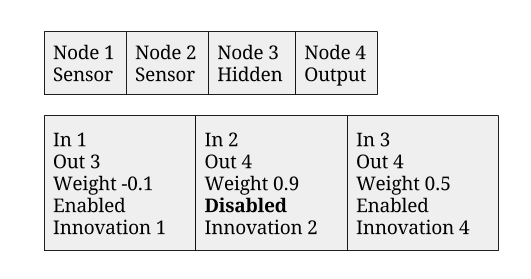
\includegraphics[width=190px]{img/genotype.png}
	\caption[NEAT gene encoding]{An example of a gene encoding of an ANN in NEAT}
	\label{fig:genotype}
\end{figure}

\subsubsection{Speciation}
Speciation in NEAT allows networks with very different topologies to compete, breed and evolve among other networks with largely the same topology.

A new topological innovation in a TWEANN, occurs when a structural change happens, like a new node or a new connection. Such a change is however likely to make the network perform considerably worse than before, compared to the networks in the population, which did not get such a significant change. In order to preserve new innovations, the entire population split into separate species, depending on their topology and they compete, primarily, within their own specie. This way, if a new innovation is placed in a new species, it will be allowed to evolve and tune its new structure to something fitting, and not just be discarded as a bad evolutionary step before it has even been explored.

The following formula is used to calculate the distance between genes for assigning species: 

$$\delta = \frac{c_1E}{N} + \frac{c_2D}{N} + \bar W c_3$$

The formula uses the number of excess genes, $E$, disjoint genes, $D$, and the average weight of the matching genes, $W$. The importance of these three parameters can be adjusted using the three variables $c1$, $c2$ and $c3$, while N is the total amount of genes in the larger of the two networks. There are no definitive optimal settings for these parameters, they have to be experimented with on a case by case basis. The goal of the parameters are to protect innovative changes as they adjust their weights to discover the potential of the change while also discarding structures which have proved not to work. \todo{What is the goal of the adjustment of these hyper parameters? When a innovative change is made, it should be protected}

At each evolution step, a random genome in a species is selected to be that specie's representative, and all other genomes get their distance calculated with regards to that genome, to determine if it should be part of that species. If a genome is too far from any species, then it will be placed in a new species where it, itself will become the representative genome.

All genomes have their fitness changed, depending on how big the species it is part of is, and how different the genomes is from the other genomes in the species:

$$f_i' = \frac{f_i}{\sum^n_{j=1} sh(\delta(i,j))}$$

$f'i$, is the modified fitness of the network, $sh(\delta(i,j))$ is a function returning 1 if $\delta(i,j)$, the distance between the networks, is below the threshold $\delta_t$, otherwise it returns 0. This results in the modified fitness being lower the larger the species the genome is part of is meaning that larger species will have to perform better in order to survive as a large species.

\subsubsection{K-Means speciation} 
\todo{how should this be cited?}http://sharpneat.sourceforge.net/research/speciation-kmeans.html
The framework used for the experiments in this paper does not use the exact speciation strategy described here. It uses K-Means Clustering for speciation which is an algorithm for distributing data points into $K$ different clusters, or in this case, species. The algorithm works by first distributing all genomes into $k$ a random clusters. Then it calculates the centre point for each cluster and continues to distribute all the genomes into the nearest cluster. If a genome has changed cluster during the re-distribution, the algorithm starts again from calculating the centre point of the clusters as they are then and distribute the genomes again. This is done until all clusters are stable or some amount of iterations.

The center point of a cluster is calculated with euclidean distance as the componentwise mean of all the points in a cluster\todo{allowed?}.

K-Means implementation uses a vector of a genes' connection's innovation ids and their weights to represent them in the coordinate system. Manhattan distance is used as the distance metric, which is not much different from the distance metric in the original speciation idea. Manhattan distance in the original distance metric is equal to ${c_1E}$ and ${c_2E}$ set to 0 and $c_3$ to 1.

\subsection{Gradient descent}
Gradient descent is an optimisation method that fits a model to a number of training examples, to learn the underlying data pattern, by minimising a cost function. In the context of image recognition, a training example is an image and associated features, such as the class that the image belongs to. The associated features are referred to as ground truths. The model subject to optimisation is an ANN.

In contrast to NEAT, gradient descent does not adjust the topology of the network. Hence, it is given a predefined topology and thus a set of parameters, known as $\theta$, which is the set of biases of all neurons and weights of all connections in the network. 

Gradient descent iterates through the set of training examples, and calculates cost through backpropagation based on the difference between the predicted features, $a(x)$, and the ground truths, $y(x)$. Euclidean loss is a common cost function.
$$C(x) = {\lVert y(x) - a(x) \rVert}^2$$
The parameters of the network are updated based on the gradient of the cost function $\nabla C$ with respect to $\theta$. By knowing the gradient with respect to every parameter of the network, the parameters can be updated, such that the cost is reduced. Consider a change in cost, as described by the change in a parameter:
$$\Delta C \approx \nabla C \cdot \Delta v $$
If the change in the parameter, $\Delta v$, is chosen, such that $\Delta v = - \eta \nabla C$, where $\eta$ is the learning rate, then it can be shown by substitution that $C$ is reduced.

$$\Delta C \approx - \eta {\nabla C}^2 $$
The learning rate is a small positive number, usually in the range of $10^{-6}$ to $1$. If the learning rate is sufficiently small, then the cost is reduced at every parameter update, but if it set too high, then $\Delta C \approx \nabla C \cdot \Delta v $ is an inaccurate approximation of the change in cost, and the parameter update might result in a rise in cost. \newline

The Euclidean loss cost function presented earlier applied to a single training example. The objective of gradient descent can be described as minimising the average cost for all training examples.

$$C_{Euclidean} = \frac{1}{n} \sum_{x} {\lVert y(x) - a(x) \rVert}^2$$

The true gradient of $C$ is approximated by averaging the gradients calculated from one or more training examples. If parameters are updated from a gradient approximated from one example, the optimisation method is known as stochastic gradient descent. If it is approximated from a number of training examples less than the total number of examples, it is known as mini-batch gradient descent. Mini-batch gradient descent is usually preferred in practice, as it is a good compromise between computational efficiency and accuracy.

\subsubsection{Cost functions}
\label{sec:negative}
For classification tasks, where the output is a probability distribution summing to one, the negative log likelihood is used as cost function. Training examples of classification tasks are represented as a binary vectors, with 1 in the class that the input belongs to. Let $y_{ij}$ be the $j$'th term of the feature vector of the $i$'th training example, and $p_{ij}$ be the corresponding prediction from the network subject to training, then the log likelihood function can be described as:
$$ C_{loglikelihood} = -\frac{1}{n} \sum_{i} \sum_{j} y_{ij}\text{ln}(p_{ij}) $$
Where $n$ is the number of training examples. Explained in more simple terms, the cost of a probability distribution is exactly equal to the negative natural logarithm of the predicted probability of the correct class. Negative log likelihood is preferred over Euclidean loss for classification tasks, as it makes gradient descent converge to the optimal solution faster\cite{Solla}.

The Euclidean loss function described in the last section is used for regression tasks, where any output sum and any output range is allowed.


\subsubsection{Momentum}
Gradient descent, as described above, can be thought of as a ball rolling down a hill until it cannot go any further. However, the speed of the ball is only proportional to the steepness of the curve, and does not accelerate like its physical analogy. While adhering to the laws of physics should not be a motivation in itself, the idea of acceleration in gradient descent has two advantages. It reduces the chance that the ball gets stuck in a local minimum of the cost function, as the momentum of the ball allows it to roll over small hills of the cost function. Secondly, it reduces the number of time steps required to roll down to the bottom of a deep valley. The momentum rules used by Nesterov's Accelerated Gradient (NAG) are slightly different from classical momentum, as it modifies the velocity based on a future position of the ball, rather than the current position. NAG performs an update to the parameters based on the velocity:
$$\theta_{t+1} = \theta_t + v_{t+1}$$
In the non-modified version of gradient descent, the velocity was only based on the gradient. NAG modifies the velocity based on the previous velocity:
$$v_{t+1} = \mu v_t - \eta \Delta C(\theta_t + \mu v_t)$$
Where $\mu$ is a hyperparameter that determines the amount of momentum. It can be shown that NAG converges faster than gradient descent for differentiable and convex cost functions.

\subsubsection{Regularisation}
\label{sec:regularisation}
Regularisation in gradient descent helps preventing the model from overfitting to the training examples. Overfitting occurs, when the optimisation method reduces the models generalisation capabilities, but increases its capabilities of correctly predicting training examples. It occurs as minimising the cost function for the training examples is only an approximate representation of the goal of gradient descent,  the true goal is to make the model generalise. When gradient descent reaches a certain point in training, the only way to get a lower cost is to overfit to the training examples. Early stopping is a strategy to reduce overfitting, by measuring the models generalisation strength on a data set not used during training.

The number of free parameters in a fully connected ANN can be high, as the number of connection weights between to layers are equal to the product of the number of neurons in each layer. A greater number of free parameters increases the overfitting potential of the model, while a greater number of training examples has the opposite effect.
High weights are indicators of overfitting, as an overfitted network detects few unique features of a single example and lets them determine the entire output, to form a "memory" from the parameters. Consequently, both l1- and l2-regularisation limits overfitting by reducing the magnitude of the weights. They do so, by adding a second term to the cost function, such that the change in parameters are influenced by the magnitude of the parameters. Let $C_0$ be the original cost function, then the cost function with l2 regularisation is,
$$C = C_0 + \frac{\lambda}{2n}\sum_{w} w^2 $$
where $\lambda$ is a hyper parameter that dictates the strength of the regularisation. l1 regularisation is very similar, the only difference being that the weights are not squared.

Overfitting can be prevented in other ways. The more training examples gradient descent uses, the less likely overfitting becomes. In the problem domain of this project, training data is readily available, and optimising with additional training data is enough to eliminate overfitting\todo{Ref to results}.

\subsubsection{The vanishing gradient problem}
\label{sec:vanishinggradient}
The vanishing gradient problem is a common problem in deep learning. To understand the solution to the problem, it is necessary to understand some details of the way backpropagation calculates the gradient of the cost function.
Backpropagation works by calculating the error of every neuron, and recursively using the error of the previous neuron to estimate the error of the next error, going backwards. The error of a neuron in the output layer is calculated as: ${\delta}_a = C_a \nabla \cdot f'(z)$. The error of the neurons in the next layer is based of a product of the derivative of its activation function. The point is, that the further the error travels backwards in the network, the more derivatives gets included in the product. If the derivative is small, the error gets small as well, which leads to small updates to the parameters, which finally leads to slow learning. The sigmoid activation function has an output range of $[0,1]$ and the derivative is calculated as $s'(z) = s(z) \cdot (1-s(z))$. It is apparent that the largest value of $s'(z)$ is $\frac{1}{4}$, and that the derivative gets small in the edges of the range. For examples, in 12 layer network, the error would in the best case scenario be multiplied by ${\frac{1}{4}}^{12} \approx 5.96 \cdot 10^{-8}$. Consequently, this activation function would result in very slow learning in the lower layers. The rectifier activation function partially solves this problem by having a derivative of:
\[
    f'(z) =  
\begin{dcases}
    1,& \text{if } z > 0\\
    0,              & z \leq 0
\end{dcases}
\]
This allows the error to persist through the layers. However, the error is canceled entirely if $z$ is below zero, and the vanishing gradient problem still persists to some degree. If the initialisation of the network results in a ReLU function outputting exclusively zero for all the training examples, it dies and is useless. Consequently, avoiding dying units in the output layer might require multiple initialisations with different seeds. Google's LeNet \cite{christian} additionally addresses the vanishing gradient problem by having multiple output layers calculating outputs from only a subset of the network, thereby reducing the number of steps that the error travels to reach the lowest layers of the network.

\subsubsection{Xavier initialisation}
The initial values of the weights of the network is important when training deep neural networks. Too low weights causes the error signal of backpropagation to stagnate, and too high weights causes the weighted input sum, $z$, to become too large or too small. It is desirable to let be $z$ within a low range, as the non-linearity of the activation function is centered at zero.
Drawing the weights from a normal distribution with a mean of zero and a constant variance does not necessarily keep the weights within the desired range, as the number of inputs varies from neuron to neuron. A neuron with a thousand inputs have a larger variance on its weighted input sum than a neuron with ten inputs, if they both use the same variance.
Xavier et al. \cite{DBLP:journals/jmlr/GlorotB10} suggests an initialisation, where the variance is based on the number of input and output signals, respectively denoted $n_{in}$ and $n_{out}$.
$$ \text{Var}(W) = \frac{2}{n_{in} + n_{out}} $$
This helps keep the weights within a range that makes gradient descent converge faster than with a constant variance.

\subsubsection{Distribution imbalance in classification training data}
\label{sub:data-req}
According to recent research~\cite{balanced-classes} having imbalanced representations of classes used for training with gradient descent can lead to poor performing networks. According to the study, the worst cases of networks trained on imbalanced data were only able to consistently classify images belonging to the most represented class, i.e. one out of a total of ten classes. The imbalance of data were at most a factor of two, i.e the most represented class having twice as many samples as the least represented class.

The complications introduced by imbalanced class distributions can be addressed by evening the distribution of classes. Overcoming the imbalances can be achieved through different approaches.

One method is to delete data from over-represented classes until every class has an equal amount of samples. This can severely affect the amount of training data as data is deleted until every class has samples equal to the lowest denominator.

A second method is proposed in~\cite{balanced-classes}, showing promising results. The idea is to randomly duplicate samples from lesser represented classes, until classes are more evenly distributed. The most extreme form of this method duplicates samples until an even distribution is obtained.
\subsection{Related work}
\label{sec:relatedwork}
In 2014, a visual agent for playing TORCS\footnote{The Open Racing Car Simulator} was developed using reinforcement learning to evolve a network with a CNN component\cite{torcs}. The fitness functions used to train the top layer network was different than the fitness function used to train the CNN component. The top layer network adapted the output of the CNN component and successfully used it, despite the output of the CNN component being humanly incomprehensible, and based solely on the image. The TORCS AI demonstrates the strong input interpretation potential of NEAT.

Chenyi Chen et al. \cite{chen} trained a deep convolutional neural network to detect features of road images in TORCS, retextured to simulate real driving. The features included angle of the road tangent and distance to land markings. The features were translated to driving actions by a handwritten controller, which is the main difference between their and our approach. The advantage of their approach is that the desired behaviour of the agent can be formulated in detail, which is necessary when programming critical systems, like an autonomous car.

The real time shooter Doom has seen several successful AI implementations using convolutional neural networks with reinforcement learning in the Visual Doom AI competition, as for example by Michal Kempka et al.\cite{vizdoom} and Lampre et al.\cite{DBLP:journals/corr/LampleC16}. The domain are similar to ours, but the training methodology differs. Many of the top performing entries for the competition used deep reinforcement learning to estimate the Q-value of states. The networks were trained with stochastic gradient descent with data labeled by reinforcement learning. This way of controlling the agent is quite different from out approach, as it is based on a state representation of the game and does not utilize neuroevolution.

Deep reinforcement learning has been applied to several different games, using  high dimensional sensory output, such as images. Volodymyr Mnih et al.\cite{DBLP:journals/corr/MnihKSGAWR13} uses deep reinforcement learning to play 9 different Atari 2600 games, achieving state of the art results in 6 of them. One of the advantages of this approach is that it is independent of the feature representation, which can be a challenge to design manually. However, deep reinforcement learning does not perform well on games requiring long term strategic planning.

Numerous examples of applying supervised learning or evolutionary algorithms to FPS games exist\cite{benjamin}\cite{silvano} and neuroevolution is frequently applied to games of other genre, as outlined by Sebastian Risi et al.~\cite{DBLP:journals/corr/RisiT14}. Some of the examples uses HyperNEAT to deal with relatively high dimensional input\footnote{16x21 for Atari and 7x7 for Go, compared to 256x256 images used in this project.}, as HyperNEAT can evolve repeating connection and topological patterns. Few of the examples, uses the visual partially-observable state. This difference is not only significant in terms of the methods required to solve the problem, but also in terms of the expected behaviour of the agent.

\subsection{The FPS setting}
\label{sec:fpssetting}

The FPS environment used as a test bed for the pipeline is described in this section. The agent starts with a single full automatic weapon, which has 30 bullets in a single magazine. It has 6 extra magazines at its disposal. The weapon does not automatically reload when the magazine is empty, in order to force the agent to learn detecting when a magazine is empty. Since the agent does not get any input regarding bullets and magazines left, it should, optimally, learn to count how many bullets and magazines it has used. This is important in order to not waste time attempting to shoot or reload when there are no more bullets or the weapon is fully loaded, it is however possible to get very reasonable behaviour from the agent without perfect reload times.

The target spawns with 100 health points, and a single bullet does 10 damage to it, no matter where it hits. This means that 10 hits are required for the agent to kill the target. If the the agent only reloads when it is out of bullets, it will have 210 bullets, meaning it could theoretically eliminate 21 targets. The agent is however not given enough time to eliminate such a high number of targets, but it is given plentiful extra bullets, to allow for mistakes, in order to increase the learning rate.

The weapon has a violent recoil which the agent has to learn how to control. The recoil is set to miss the enemy/bot already on the third shot in far the most cases and emptying an entire magazine will on average hit the target 3-4 times. As this will result in a very low score, the agent will have to learn how to control the recoil. The recoil is random, so the agent has to learn how to tap-fire in order to maximise accuracy. Had the recoil not been random, as it is seen in games like Counter Strike, then the optimal agent would learn the exact pattern and move and shoot so that all bullets hit the bot as fast as possible. The weapon can shoot 10 times per second.

The arena the agent learns in is quadratic, with the agent spawning on one side and the targets spawning on the other, as seen in figure \ref{fig:arena}. Both the agent and the target spawn in a random x and y, while the z coordinate is constant. The first target in the arena always spawn within sight of the agent in order to improve the learning rate. The arena is outfitted with 3 lights to create different visual representations of the target. One light is in the middle of the agent side in order to create differing lightning images of how the agent sees himself. The other two lights are placed on the side of the target, in a way which provide very varied light settings on the target, to test the VRC under different conditions.

\begin{figure}[H]
	\centering
	\begin{scriptsize}
		\sffamily
		\input{img/arena.pdf_tex}
	\end{scriptsize}
	\caption[The FPS game arena]{The arena as seen from above. This illustration omits the y-axis. The lines represent planes, as the agent and the target spawns randomly along both the y-axis and the x-axis.}
	\label{fig:arena}
\end{figure}




















































    %!TEX root = ../preamble.tex

\section{Solutions}
\label{sec:solutions}
Creating a fully functional visual FPS agent requires solutions to a range of different problems. To narrow the scope of the solution, the functionality of the proposed solutions is limited to only a subset of the required functionality to play a full-fledged FPS game, as Counter Strike or Quake. Developing a FPS agent capable of playing like a human player requires the following functionality:
\begin{itemize}
\item Movement - The agent can move efficiently between points of interest.
\item Navigation - The agent can recognise different maps and utilise strategic positions.
\item Aiming and shooting - The agent can identify targets, aim and shoot efficiently with a range of weapons.
\item Identification of objects of interest - The agent can identify objects of interest, such as armour, weapons and flags.
\item Identification of sound - The agent can identify threats from sound.
\item Adaption of role in a team - The agent can identify the roles of its teammates and are able to put itself in a position that compliments the team.
\end{itemize}
The focus of the solution is aiming and shooting, and the proposed solutions only attempts to solve this problem.

\subsection{Granularity of control}
The frequency of which the AI makes decisions is a parameter that shapes the potential and performance requirements of the solution. The finest level of control is achieved by parsing every single frame of the game to infer an action. This is performance intensive, as the process of parsing the visual output through the VRC requires significant amount of computational resources. Using a control frequency lesser than the number of frames reduces the potential reaction speed of the agent and the overall smoothness of its behaviour. The approach of Michal Kempka et al.\cite{vizdoom} is also vision based, and repeats the chosen action for $k$ frames. We chose the same approach, as the flexibility of skipping frames reduces the hardware requirements.
Some of the functionality requirements of an agent capable of playing a game like Counter Strike might require higher level of control, such as deciding the long term strategy plan or navigating larger maps. This is not in the scope of the proposed solutions.

\subsection{Actions}
The agent should be able to aim, shoot and reload. Therefore, the output of the AIC is turn horizontally, turn vertically, shoot and reload. The turn actions are analog, such that the greater the output, the faster it turns. Shoot and reload are binary actions, that triggers when the output is above a specific threshold. Shooting takes precedence over reload, and turning can be done while shooting or reloading.

\subsection{Feature representations}
Recall that the feature representation is the integration point of the VRC and the AIC, and that it is the output of the VRC and the input of the AIC.
The feature representation of the visual state should allow the AIC to locate an enemy, aim and shoot it, while having as few dimensions as possible, as the evolution speed is a central concern. Additionally, the VRC has to be able to learn the features from training examples.

\subsubsection{Angular representation}
\label{sec:angular}
The angular feature representation unambiguously defines the position of the target on the screen. This representation has two angles, a distance and a binary output indicating whether the target is within sight. Figure \ref{fig:angular} shows the vertical angle, given by the angle between the current facing of the agent and a projection of the vector from the agent to the target. The projection is onto a plane determined by the vector of the current facing and the up-vector.
\begin{figure}[H]
    \centering
    	\begin{scriptsize}
		\sffamily
    	\includesvg[svgpath = img/, width = 0.7\textwidth]{verticalangle}
    	\end{scriptsize}
    \caption[Calculation of angles]{The relative vertical angle.}
    \label{fig:angular}
\end{figure}
\noindent
The horizontal angle is calculated in the same manner, except that the angle is calculated based on the projection of both vectors onto the horizontal plane. These two angles allows the AIC to infer the aiming directly. The distance is included to allow for changing shooting behaviour based on distance. For example, if the agent shoots a full automatic rifle at a long distance, it might be better to fire separate shots than using automatic fire. The binary indication of whether there is a target within sight, has the purpose of clarifying whether the angles reflects the position of a target, or just assumes default values.
\begin{figure}[H]
    \centering
    	\begin{scriptsize}
		\sffamily
    	\includesvg[svgpath = img/, width = 1\textwidth]{angular}
    	\end{scriptsize}
    \caption[Angular representation of the visual state]{The vertical and horizontal angles define a position on the screen. The field of view is $65^\circ$ and the target is at a horizontal angle of $-17.17^\circ$ and a vertical angle of $15.05^\circ$ in this example.}
    \label{fig:angular}
\end{figure}

\subsubsection{Visual partitioning representation}
\label{sec:vpr}
The visual partitioning representation ambiguously indicates the position of the target on the screen. It defines the position of the target as a classification task, where each point on the screen belongs to a class bounded by a square as shown in figure \ref{fig:visualpartitioning}. 
\begin{figure}[H]
    \centering
    	\includesvg[svgpath = img/]{visualpartitioning}
    \caption[Visual partitioning representation]{The position of the target is interpreted as the square of which his centre of mass(marked by the blue dot) is located.}
    \label{fig:visualpartitioning}
\end{figure}
\noindent
As the target can be visually present in multiple squares, the correct square is defined as the square that contains his centre of mass. The partitioning is finer in the centre of the screen to allow for fine adjustments of the aim. The notation of the partitioning scheme is defined as the number of partitions on the vertical and horizontal axis of the whole screen, followed by the number of partitions on the horizontal or vertical axis of the centre of the previous partitioning. The scheme is exemplified in figure \ref{fig:visualpartitioningcompared}.

The feature representation is a sparse vector with a term for each partition. The term of the partition that contains the target is one, while all others are zero. If no partition contains the target, an additional term indicates the absence of a target.
\begin{figure}[H]
    \centering
    	\includesvg[svgpath = img/, width = 0.8\textwidth]{visualpartitioningcompared}
    \caption[Partitioning schemes]{The leftmost partitioning scheme is notated 3,3,3 and the rightmost is notated 5,3.}
    \label{fig:visualpartitioningcompared}
\end{figure}

\subsubsection{Optimal visual partitioning scheme}
The optimal visual partitioning scheme depends on many factors. It is necessary that a part of the target is present in the exact centre of the image, if the position of the target is classified as the centre partition. In that situation the agent would always, assuming no recoil, hit the enemy if there is an enemy in the centre partition and the agent shoots. Without that guarantee the task of consistently shooting the enemy becomes more difficult. The agent receives no feedback from misses, consequently if the centre square is to large, it can become impossible for the agent to learn to hit. The size of the agent is depending on distance, and this requirement is therefore depending on the distance that the agent should be able to hit at.

Assuming the target is 11 pixels wide and has a box-shaped hitbox\footnote{The projection of the target onto the screen that registers as a hit when shot at}, having a centre square of 11x11 pixels would fulfil the aforementioned requirement. If $6/11$ pixels is inside the centre square the enemy is considered to be inside that partition and since the sixth pixel is the centre pixel of the centre square, a part of the enemy is in the centre of the centre square - fulfilling the requirement.

A 5, 3 partitioning scheme would result in the centre partition being around 17 pixels wide, where it for a 3, 3, 3, partitioning scheme is approximately 9 pixels wide. There are 34 classes using a 5, 3 partitioning scheme, calculated as $(5*5-1)+(3*3)+1=34$ and 26 classes using a 3, 3, 3, partitioning scheme, calculated as $(3*3-1)+(3*3-1)+(3*3)+1=26$.

Since a 3, 3, 3 partitioning scheme results in fewer classes than a 5, 3 partitioning scheme, leading to faster training of the agent, and the resulting width of the centre partition is narrower, all experiments were done using a 3, 3, 3 partitioning scheme.




\subsubsection{Comparing the representations}
The feature representation of the VPR(visual partitioning representation) has a significantly larger number of dimensions(26 for 3,3,3 partitioning compared to the 6 of angular) than the angular representation, consequently slowing down evolution. The VPR is less detailed, as the precision of the angular representation is bound by the precision of the decimal used to represent the angle, while the precision of the VPR is bound by the width of the partitions. The angular representation allows the agent to choose shooting strategy based on distance and generally allows the agent to behave more smoothly. The large partitions of the VPR in the edges of the screen provide very ambiguous information about the position of the enemy, which makes it impossible for the agent to evolve smooth human-like aiming. If the agent was allowed to move or take strategic decisions, this lack of detail might reduce the potential of the agent furthermore. The angular representation allows the agent to aim precisely, which many FPS shooter games rewards by increasing the damage inflicted for hitting vulnerable areas on the target.

The only advantage of the VPR is that it is significantly easier to train a CNN to recognise this representation than the angular representation.

\subsection{The topology of the convolutional neural network}
The topology of the CNN has lots of different optimisation parameters, and as hyperparameter optimisation methods are based on trial and error, it takes time and computational resources to optimise. The project inevitably leaves room for better topologies that performs better, and the search for an efficient topology is not in the scope of this project. However, we impose some requirements on the topology. The stack of convolutional layers has to have a receptive field that can detect the target, as explained in section \ref{sec:topologies}. The width and height of the target is depending on distance, but it is approximately 10 pixels wide and 25 pixels high. Therefore, the topology of the network should be able to recognise visual features spanning at least 25 pixels. The network should have some depth, as it is often correlated with better performance\cite{christian}\cite{karen}, and use the rectifier activation function to reduce the vanishing gradient problem as described in section \ref{sec:vanishinggradient}.






































	%!TEX root = ../preamble.tex

\section{Approach}
\label{sec:approach}
To answer the research question from section~\ref{sub:research-question}, we train a CNN as well as an ANN with neuroevolution, combine them and run varying experiments. This section describes the details of how the networks subject to experimentation are trained and combined.
\todo{read source comment}
%This section needs structure. We need to decide on large subsections. Maybe these 3: Training the CNN; Evaluation for neuroevolution; Combining... feel free to rename

\subsection{Training the convolutional neural network}
This section describes the details of the training of the CNN, including the training examples, the network topology and the hyperparameters. 

\subsubsection{Topologies}
We present four different topologies, two for classification and two for regression. Both types are tested with a 12 layered architecture and a 6 layered architecture, called deep and shallow respectively. The difference between the two topologies is in the number of neurons in the fully connected layers and in the activation functions used for the output. All activation functions are ReLU(rectifier), except in the output layers, where softmax is used for classification and identity is used for regression. The regression network outputs the angular representation as described in section \ref{sec:angular}, scaled to fit a range of $-1$ to $1$. The classification network outputs 26 probabilities summing to $1$. The networks take inputs with a shape of 256x256x3, which is the 3 color channels of the image.

\paragraph{Deep neural network topologies}
The network topologies are illustrated on figure \ref{fig:architectureOfDeepNet}. Both have 12 layers, the first 8 being alternating convolutional and pooling layers, while the next 3 layers being fully connected layers followed by an output layer.  The stride and zero padding of all the convolutional layers are 1, while the stride of all the pooling layers is 2. Both networks have a total of 3,200 parameters(weights and biases) in the convolutional layers.
The classification network has 1,228,800 weights($16 \cdot 16 \cdot 120 \cdot 40$) from the last convolutional layer to the first fully connected layer and 4,386 parameters in the remaining layers.
The regression network has 7,680,000 weights($16 \cdot 16 \cdot 120 \cdot 250$) from the last convolutional layer to the first fully connected layer and 126,754 parameters in the remaining layers.

\begin{figure}[H]
	\begin{scriptsize}
		\sffamily
		\def\svgwidth{\textwidth}
		\input{img/architectureOfDeepNet.pdf_tex}
	\end{scriptsize}
	\caption{The full topology of the deep convolutional neural networks.}
	\label{fig:architectureOfDeepNet}
\end{figure}

\paragraph{Shallow neural network topologies}
The network topologies are illustrated on figure \ref{fig:architectureOfShallowNet}. Both have 6 layers, the first 4 being alternating convolutional and pooling layers, followed by a fully connected layer and an output layer.  The stride and zero padding of all the convolutional layers are 1, while the stride of all the pooling layers is 4. Both networks have a total of 5200 parameters(weights and biases) in the convolutional layers.
The classification network has 3,686,400 weights($16 \cdot 16 \cdot 120 \cdot 120$) from the last convolutional layer to the first fully connected layer and 3,266 parameters in the remaining layers.
The regression network has 23,040,000 weights($16 \cdot 16 \cdot 120 \cdot 750$) from the last convolutional layer to the first fully connected layer and 3,754 parameters in the remaining layers.

\begin{figure}[H]
	\begin{scriptsize}
		\sffamily
		\def\svgwidth{\textwidth}
		\input{img/architectureOfShallowNet.pdf_tex}
	\end{scriptsize}
	\caption{The full topology of the relatively shallow convolutional neural networks.}
	\label{fig:architectureOfShallowNet}
\end{figure}

\subsubsection{Training with gradient descent}
The optimisation process of gradient descent did not include continuous evaluation on a validation set for early stopping, as overfitting was of no concern. When the error of the network stopped improving, the process was stopped. The parameters were updated from a mini-batch of size 32, with a learning rate of $10^{-3}$. The process did not include dropout, but included L2-regularization with a coefficient of $5 \cdot 10^{-4}$ for some of the experiments. Nesterov's accelerated gradient was used with a momentum coefficient of $0.9$. The networks were initialised with Xavier initialisation. The number of training examples used for training was 130,000 for all experiments. The framework used for supervised learning was DL4J, a deep learning framework for java, accessable at \url{https://deeplearning4j.org}.

\subsubsection{Training data}
The training examples consists of the raw image data and ground truths. The raw image data is, for each pixel, the byte value of the red, green and blue pixel, i.e. three numbers between 0-255, arranged as a 3 dimensional volume, as seen in figure \ref{fig:split}.

\begin{figure}[H]
    \centering
    \includesvg[svgpath = img/]{RGBtransformation}
    \caption{An image split into its three color channels.}
    \label{fig:split}
\end{figure}
\noindent
The ground truth is different for the visual partitioning representation and the angular representation. For the VPR it is a vector with a 1 in the correct class, and for the angular representation it is a 4 dimensional vector with the correct representation.
In section~\ref{subsub:data-gen} it is explained how the training data for this project was gathered.


\subsubsection{Binarisation of the visual partitioning representation}
The output of the CNN approximating the visual partitioning representation is a probability distribution summing to 1, as described in section \ref{sec:vpr}. When the CNN is used as input provider to the evolved ANN, output of the CNN is transformed to a sparse vector with a 1 in the class with the highest probability. This makes the input similar to the input that the evolved ANN is trained with.

\subsubsection{Scaling of the angular representation}
The angular representation of the position of the target consists of four dimensions as described in section \ref{sec:angular}. The horizontal and vertical angle are scaled to $[-1,1]$, the distance is divided by $20$, and the bit indicating whether the target is within sight is either 1 or 0. When the angular representation is estimated by a CNN and used as input to the evolved ANN, angles are cutoff if they are outside the range of $[-1,1]$, and the indication of whether a target is present is rounded to 0 or 1. If the indication is rounded to 0, the other dimensions are set to 0 for consistency, regardless of the output of the CNN.

%\subsection{Visual partitioning}
%To train the CNN to be able to classify images, classes are needed. Two obvious classes are pictures with and without an enemy. Having only these classes does not provide enough information for NEAT to be able to produce intelligent behaviour. In other words, more classes are needed.
%\todo{Basically already explained in section solutions}
%Introducing more classes is achieved by splitting the image into partitions, where an image belongs to a class if there is an enemy in the corresponding partition.

%Figure~\ref{fig:image-partition}\todo{insert figure} shows an example image that has been split into nine squares. The centre square has been further split into nine squares as well. This partitioning scheme is called a 3, 3 partitioning scheme as the image is split into three squares both horizontally and diagonally, and the same is done to the centre square.

%A 3, 3, 3 partitioning scheme is almost the same as before, except the centre square is further split into three squares both horizontally and diagonally.

%Using a 3, 3, 3 partitioning scheme results in 26 different classes. This is calculated as $(3*3-1)+(3*3-1)+(3*3)+1$. One is subtracted from $(3*3)$ in the first two occurrences, as their centre square is further partitioned. The $+1$ in the end is the class that states there is not an enemy in the picture. The 25 other classes are images where an enemy is in one of the 25 different partitions.

% SKRIV VIDERE

%%!TEX root = ../preamble.tex

\newcolumntype{M}[1]{>{\centering\arraybackslash}m{#1}}

\def \emptyLine{\multicolumn{3}{| c |}{}  & \multicolumn{3}{c |}{}  & \multicolumn{3}{c |}{}}

\renewcommand{\arraystretch}{1.9}

\includegraphics[height=256px]{img/134.png} \vspace*{-260px}

\begin{figure}[H]
\color{black!50}
\begin{tabular}{| p{28px} | p{28px} | p{28px} | p{28px} | p{28px} | p{28px} | p{28px} | p{28px} | p{28px} |}
\hline
	
	\multicolumn{3}{| p{84px} |}{\multirow{3}{*}{}} &
	\multicolumn{3}{  p{84px} |}{\multirow{3}{*}{}} &
	\multicolumn{3}{  p{84px} |}{\multirow{3}{*}{}} \\
	\emptyLine \\
	\emptyLine \\
	
\hline
	
	\multicolumn{3}{| c |}{\multirow{3}{*}{}} &
	& & &
	\multicolumn{3}{  c |}{\multirow{3}{*}{}} \\ \cline{4-6}
	
	\multicolumn{3}{| c |}{}  &
	& & &
	\multicolumn{3}{c |}{} \\ \cline{4-6}
	
	\multicolumn{3}{| c |}{}  &
	& & &
	\multicolumn{3}{c |}{} \\

	
\hline
	
	\multicolumn{3}{| c |}{\multirow{3}{*}{}} &
	\multicolumn{3}{  c |}{\multirow{3}{*}{}} &
	\multicolumn{3}{  c |}{\multirow{3}{*}{}} \\
	\emptyLine \\
	\emptyLine \\
	
\hline
\end{tabular}
\caption{Example partition of the screen using a 3, 3 partitioning scheme}
\label{fig:image-partition}
\end{figure}


%Having a fully automated process of producing pixel data and labels allowed different arena setups to be tested quickly.

%The data was saved in a database to make it possible for multiple computers across different networks to both retrieve from and persist to the database.

\subsection{Training the agent}
\label{sub:training-neat}
The agent was trained with a modified version of NEAT as described in section \ref{sec:neat}\todo{describe the sharpNEAT framework}. The training of the agent was done in Unity 5\todo{link?}, using the UnityNEAT framework\todo{https://github.com/lordjesus/UnityNEAT}, which is a, slightly modified, implementation of NEAT and made easy to use with games developed in Unity.
Training the agent using the CNN as the ground truth provider is extremely computationally heavy using the setup of this project and therefore not feasible. Having access to more computational resources or more low level control with the hardware might overcome these challenges. Since neither was available at the time of writing, the CNN was not used as the ground truth provider. Instead of having the CNN detect which visual partition the enemy is in, it is calculated using the state of the game. This method is far less computationally heavy, making the training of the agent a lot faster.

\subsubsection{Evaluation}
The fitness of a network was evaluated in the FPS game described in section \ref{sec:fpssetting}. An evaluation lasts 15 seconds, and as the evaluation includes some randomness, each evaluation was repeated 20 times and the results averaged. The random spawn of the target, and agent, ensures that the agent does not learn a specific pattern, but learns to act in any situation. The agent was awarded for hitting the target and aiming closer to the target.

\subsubsection{Fitness function}
The fitness function for the evaluation can be formulated as:
$$f = \text{damage} + \text{aim\_bonus}$$
Where damage is the total damage dealt, and aim\_bonus is calculated as:
$$ \text{aim\_bonus} = \frac{1}{n} \sum_{n} \frac{c}{(1+v)^2} $$
Where c is a constant set to 75, $n$ is the number of frames and $v$ is the angle measured in radians between the forward pointing vector of the agent and the line from the agent to the target. Hence $v = 0$ if the agent aims directly at the target. This bonus makes the evolution faster, as dealing damage requires aiming, and evolving the ability to aim takes several generations.
\begin{figure}[H]
\centering
\begin{tikzpicture}
	\begin{axis}[
		scale only axis,
		height=5cm,
		width=10cm,
		domain={0:3.1415926535},
		samples=30,
		xmin=0,   xmax=3.1415926535,
		ymin=0,   ymax=75,
		xlabel=$v$,
		ylabel={aim\_bonus}
	]
	% use TeX as calculator:
	\addplot[mark=none]{75 / (1 + x)^2};
	\addplot +[mark=none] coordinates {(0.7333, 0) (0.7333, 75)};
	\end{axis}
\end{tikzpicture}
\caption{The fitness awarded as a function of the angle between the current and the desired pointing direction. The red line marks the value of $v$ when the target is at the corner of the screen}
\end{figure}

\subsubsection{NEAT setup}
The hyperparameters of NEAT are shown in the table below. The activation function used is sigmoid, and biases are modelled by having a constant input, which when connected to, is the equivalent of a bias. The networks start fully connected and allow recurrent connections to appear.
%!TEX root = ../preamble.tex


\begin{minipage}{\textwidth}
\vspace{4mm}
\begin{center}

\captionof{table}{NEAT hyperparameters used to train the agent}
\label{tab:neat-hyperparams} 

	\begin{tabular}{| c | r |}
		\hline
	
		\textbf{Hyperparameter} & \textbf{Value} \\ \hline
		Population size & 100 \\ \hline
		Elitism & 20\% \\ \hline
		Asexual offspring & 80\% \\ \hline
		Sexual offspring & 20\% \\ \hline
		Interspecies mating proportion & 0.01\% \\ \hline
		Connection weight range & -5 | 5 \\ \hline
		Connection weight mutation probability & 80\% \\ \hline
		Add node probability & 3\% \\ \hline
		Add connection probability & 5\% \\ \hline
		Delete connection probability & 0.4\% \\ \hline
		Species & 10 \\ \hline
		Speciation constant C1 & 1 \\ \hline
		Speciation constant C2 & 1 \\ \hline
		Speciation constant C3 & 0.4 \\ \hline
		
	\end{tabular}
\end{center}
\end{minipage}


\subsubsection{Data generation}
\label{subsub:data-gen}
Training data representative of what the agent will encounter during actual play, will lead to better performing networks as they should not encounter anything they have not been trained for.

Taking pictures of the environment, in which the agent is during actual play, using random positioning and rotation of the camera should produce representative training data. In our case having the camera at a fixed position and random rotation should suffice as our agent is stationary.

An untrained NEAT agent, basing its actions on the angular game state, exhibits more or less random behaviour. During training the behaviour should become less random and more intelligent, which is desirable under normal circumstances, but not when the agent is used to generate training data. Disabling the fitness function, i.e. always giving a fitness of 0, disables learning, thereby persisting the random behaviour.

We were able to almost fully automate the process of generating training data by disabling the fitness function, making it possible to take a screenshot every $n$-th frame, where $n$ was around 5-10,  thereby getting a set of images representative of the states the agent would be in, during actual play.


\subsubsection{Data cleaning}
Problems can occur when representation of classes are imbalanced, as discussed in section~\ref{sub:data-req}.

To overcome these problems some of the images not containing an enemy was deleted. Before deletion approximately half of the images did not contain an enemy. We decided to delete images such that, after deletion around 15\% of the images did not contain an enemy.

The distribution of the rest of the classes depends heavily on the granularity of the partitioning scheme used. Using a 3, 3, 3 partitioning scheme, the most represented class, not counting images without an enemy, constitutes around 11\% of the images. The least represented class contained a mere 0.0862\% of the samples. In other words our representation of classes were majorly imbalanced as seen in figure \ref{fig:enemy-dist}.

Even though we had these large differences in the number of pictures from each class, the convolutional neural network was able to learn what it should, as it can be seen in our results throughout section~\ref{sec:results}, contrary to the claims of~\cite{balanced-classes}.

%!TEX root = ../preamble.tex

\begin{minipage}{\textwidth}
%\vspace{4mm}
\begin{center}

\captionof{table}{Distribution of classes of the 130,000 training samples}
\label{tab:enemy-dist} 

	\begin{tabular}{| c | r | r | r |}
		\hline
	
		\textbf{Partition} & \multicolumn{3}{c |}{\textbf{Percentage}} \\ \hline
		0 & 8.1846 \% & \multicolumn{2}{c |}{\multirow{8}{*}{72.6507 \%}} \\ \cline{1-2}
		1 & 9.2277 \% & \multicolumn{2}{l |}{} \\ \cline{1-2}
		2 & 7.8015 \% & \multicolumn{2}{l |}{} \\ \cline{1-2}
		3 & 11.6000 \% & \multicolumn{2}{l |}{} \\ \cline{1-2}
		4 & 11.3446 \% & \multicolumn{2}{l |}{} \\ \cline{1-2}
		5 & 8.0100 \% & \multicolumn{2}{l |}{} \\ \cline{1-2}
		6 & 8.6323 \% & \multicolumn{2}{l |}{} \\ \cline{1-2}
		7 & 7.8500 \% & \multicolumn{2}{l |}{} \\ \hline
		8 & 1.4000 \% & \multirow{8}{*}{11.0278 \%} & \multirow{17}{*}{12.3602 \%} \\ \cline{1-2}
		9 & 1.3715 \% & & \\ \cline{1-2}
		10 & 1.3662 \% & & \\ \cline{1-2}
		11 & 1.4131 \% & & \\ \cline{1-2}
		12 & 1.5477 \% & & \\ \cline{1-2}
		13 & 1.1777 \% & & \\ \cline{1-2}
		14 & 1.3762 \% & & \\ \cline{1-2}
		15 & 1.3754 \% & & \\ \cline{1-3}
		16 & 0.1646 \% & \multirow{9}{*}{1,3324 \%} & \\ \cline{1-2}
		17 & 0.2046 \% & & \\ \cline{1-2}
		18 & 0.1677 \% & & \\ \cline{1-2}
		19 & 0.0862 \% & & \\ \cline{1-2}
		20 & 0.1100 \% & & \\ \cline{1-2}
		21 & 0.0877 \% & & \\ \cline{1-2}
		22 & 0.1762 \% & & \\ \cline{1-2}
		23 & 0.1846 \% & & \\ \cline{1-2}
		24 & 0.1508 \% & & \\ \hline
		No enemy & \multicolumn{3}{c |}{14.9885 \%} \\ \hline
	
	\end{tabular}
\end{center}
\end{minipage}


%\subsection{Training image recognition}
%The convolutional neural network used for image recognition was trained using mini batches. A mini batch consists of $b$, where $b$ is dependent on the experiment, instances of training data randomly chosen between the set of training data constituting the training set, of size $t$.
%
%An experiment usually trains for multiple epochs, where an epoch is defined as $t/b$ iterations through the training set. One could call $t/b$ iterations through the training set, a complete traversal, but since every mini batch is composed of randomly selected instances of training data, one epoch could use the same instance multiple times and not use others at all.

















































	\section{Experiments}
\label{sec:experiments}

\subsection{Convolutional neural network experiments}
The CNNs described in section \ref{sec:approach} are measured in several ways to find out how well they work individually. Both the visual partitioning and angular representation are measured under different circumstances and with different topologies.

The VPR(visual partitioning representation) are measured by the percentage of its prediction that are correct, referred to as accuracy. The class that the CNN assigns the highest probability to is regarded as its prediction. Consequently, the whether the CNN predicts with a confidence of $51\%$ or $99\%$ does not change the accuracy, but it changes the cost.

The angular representation is measured in both accuracy percentage and absolute mean error. The horizontal angle, the vertical angle and the distance are measured in absolute mean error while the output indicating whether there is a target present on the image is measured in percentage accuracy. When the angular representation is used as input provider to the evolved ANN, the term indicating whether a target is present is converted to 0 or 1, whichever is closest. Hence the confidence of the prediction does not change its fitness as an input provider. 

To measure whether the CNNs overfits the training data, they are measured against the training set and a test set, using 10,000 samples.

\subsubsection{Visual distortion}
To measure how the network is penalised by having a varying visual representation of the target, the networks are trained with two different data sets, from two different visual settings, as seen in figure \ref{fig:light}. This is relevant, as both the real world and modern FPS games have various visual representations of targets. The textures are more detailed in the visually distorted version and the overlay of the player and the weapon is only present in this setting. The overlay fully or partially covers the target in some cases, making the recognition task harder, or even impossible.

\begin{figure}[H]
	\begin{scriptsize}
		\input{img/withLightWithoutLight.pdf_tex}
	\end{scriptsize}
	\caption{The two different visual settings.}
	\label{fig:light}
\end{figure}

\subsubsection{Different topologies}
The effect of depth of the CNN topologies described in section \ref{sec:approachtopologies} are measured in combination with the different visual game settings to assert its effect on training speed, overfitting and accuracy.

\subsubsection{Smaller training sets}
In a real world application of visual recognition, the number of training examples is often limited, as the training examples are subject to manual labeling. Hence, we measure both the accuracy of the VPR and the angular representation trained on significantly smaller data sets from the visually distorted game setting. Furthermore, overfitting is measured separately on these networks trained with smaller data sets, as overfitting gets more likely with fewer training examples. The data sets used are subsets of the training sets with 130,000 examples, and has an even distribution of VPR classes.

 
\subsection{Neuroevolution experiments}










	%!TEX root = ../preamble.tex

\section{Results}
This section describes the results of the experiments explained in section \ref{sec:experiments}.
%!TEX root = ../preamble.tex

\pgfplotsset{max space between ticks=40}

% USED FOR TARGET DETECTION ACCURACY
\pgfplotsset{target-acc/.style={%
        width=0.67\textwidth,
		height=7cm,
		enlarge y limits={abs=.625},
		xmin=0,
		xmax=100,
		axis y line*=none,
	    axis x line*=bottom,
	    xbar,
	    reverse legend,
	    legend style={at={(0.5,-0.125)},anchor=north},
	    yticklabels={
	    		{Without visual distortion,\\shallow network},
			{Without visual distortion,\\deep network},
			{With visual distortion,\\shallow network},
			{With visual distortion,\\deep network},
		},
		yticklabel style={align=right},
		ytick=data,
	    nodes near coords,
		every node near coord/.append style={
			/pgf/number format/fixed zerofill,
			/pgf/number format/precision=2
		},
	}
}

% USED FOR ANGULAR MSE
\pgfplotsset{angular-mse/.style={%
		width=0.67\textwidth,
		height=5.5cm,
		enlarge y limits={abs=0.7},
		xmin=0,
		xmax=0.2,
		axis y line*=none,
		axis x line*=bottom,
	    xbar,
	    reverse legend,
		legend style={at={(0.5,-0.2)},anchor=north},
	    yticklabels={
			{Mean horizontal error},
			{Mean vertical error},
			{Mean distance error},
		},
		yticklabel style={align=right},
	    ytick=data,
		%xtick style={draw=none},	
	    %xticklabels={,,,,,},
	    nodes near coords,
	    every node near coord/.append style={
			/pgf/number format/fixed zerofill,
			/pgf/number format/precision=6
		},
	}
}




































\label{sec:results}

\subsection{Convolutional neural network experiments}
The experiments performed are described in section \ref{sec:cnnexperiments}. Note that the time per iteration measured in the following sections is dependent on the hardware used for training. The hardware details are described in section \ref{sub:hardware} of the appendix.

\subsubsection{Visual partitioning representation}
\paragraph{Convergence}
Figure \ref{fig:score-nolight-vpr} and \ref{fig:score-light-vpr} show the convergence of the CNNs using VPR measured as the cost function on the mini-batch that the gradient is estimated from, over iterations. As the process of batch selection is random, the score is fluctuating. The cost function is negative log-likelihood, described in section \ref{sec:negative}.
The results presented are with and without visual distortion and with the network topologies described in section \ref{sec:topologies}. The shallow topology converges in fewer iterations, but both networks manage to converge to a solution. The average time per iteration for the data with visual distortion is 4,782 milliseconds for the deep network and 2,451 milliseconds for the shallow network.

%!TEX root = ../preamble.tex

\pgfplotstableread{data/nolight-vpr-shallow.dat}{\nolightVPRShallow}
\pgfplotstableread{data/nolight-vpr-deep.dat}{\nolightVPRDeep}

\begin{figure}[h]
\begin{tikzpicture}[scale=1]
	\begin{axis}[
			height=7.5cm,
%			title=Cost over iterations,
			xlabel=Iterations,
			ylabel=Cost,
			ymin = 0,
			xmin = -480,
			xmax = 12480,
			restrict x to domain=0:12000,
			xticklabel style={rotate=30},
			legend pos=north east,
		]
		\addplot+ [cred, mark=none] table [x={iteration}, y={score}] {\nolightVPRShallow};
		\addlegendentry{Shallow network}
		\addplot+ [cblue, mark=none] table [x={iteration}, y={score}] {\nolightVPRDeep};
		\addlegendentry{Deep network}
	\end{axis}
\end{tikzpicture}
\caption[Training the VRC using VPR without visual distortion]{Negative log likelihood cost over mini-batch gradient descent iterations using VPR without visual distortion}
\label{fig:score-nolight-vpr}
\end{figure} %DONE
%!TEX root = ../preamble.tex

\pgfplotstableread{data/light-vpr-shallow.dat}{\lightVPRShallow}
\pgfplotstableread{data/light-vpr-deep.dat}{\lightVPRDeep}

\begin{figure}[H]
\begin{tikzpicture}[scale=1]
	\begin{axis}[
			title=Cost over iterations,
			xlabel=Iterations,
			ylabel=Cost,
			xmin = -480,
			xmax = 12480,
			restrict x to domain=0:12000,
			xticklabel style={rotate=30},
			legend pos=north east,
		]
		\addplot+ [cred, mark=none] table [x={iteration}, y={score}] {\lightVPRShallow};
		\addlegendentry{Shallow network}
		\addplot+ [cblue, mark=none] table [x={iteration}, y={score}] {\lightVPRDeep};
		\addlegendentry{Deep network}
	\end{axis}
\end{tikzpicture}
\label{fig:score-light-vpr}
\caption[Training the VRC using VPR with visual distortion]{Negative log-likelihood cost over mini-batch gradient descent iterations using VPR with visual distortion}
\end{figure} %DONE
\vspace{-5mm}

\paragraph{Performance}
The accuracy of the results in figure~\ref{fig:vpr-acc} is measured as the percentage of correct predictions. It is apparent from these results, that the models have not overfitted to the training data, as the difference in accuracy of the training set and the test set is insignificant. Furthermore, the topologies of the networks does not seem to have a significant impact on the accuracy. Examples of the training examples that the deep CNN with visual distortion fails to classify correctly can be seen in section~\ref{sec:incorrectpredictions} of the appendix. The incorrect predictions are due to the target being in between partitions or behind the weapon overlay.

%!TEX root = ../preamble.tex

%\hspace{-8mm}
\begin{figure}[H]
\begin{tikzpicture}
\begin{axis}[target-acc]

% Test set
\addplot [draw=cgreen, fill=cgreen!70] coordinates {
	(95.33,3) % Correct value - nolight shallow
	(95.19,2) % Correct Value - nolight deep
	(85.74,1) % Correct value - light shallow
	(86.66,0) % Correct value - light deep
};

% Training set
\addplot [draw=cred, fill=cred!70] coordinates {
	(96.05,3) % Correct value - nolight shallow
	(95.94,2) % Correct value - nolight deep
	(86.10,1) % Correct value - light shallow
	(86.60,0) % Correct value - light deep
};

\legend{Test set,Training set}
\end{axis}

\end{tikzpicture}
\caption{Accuracy of partitioning classification using VPR}
\label{fig:vpr-acc}
\end{figure}













































 %DONE


\subsubsection{Angular representation}
\paragraph{Convergence}
Figure~\ref{fig:score-nolight-angular} and~\ref{fig:score-light-angular} show the convergence of the CNNs using AR shown as the cost function on the mini-batch that the gradient is estimated from, over iterations. The cost function is Euclidean loss, described in section \ref{sec:angular}.
The results presented are both with and without visual distortion and with the network topologies described in section \ref{sec:topologies}. The deep network reaches a lower cost, but requires additional iterations to converge to a solution. The deep network trained with light has an average time per iteration of 3,734 milliseconds, while the shallow network trained with light has an average time per iteration of 2,572 milliseconds. Consequently, the deep network converges significantly slower.

The same phenomena as without visual distortion is observed in figure~\ref{fig:score-light-angular}, but the difference in final cost is less than without visual distortion.

%!TEX root = ../preamble.tex

\pgfplotstableread{data/angular-nolight-shallow.dat}{\angularNolightShallow}
\pgfplotstableread{data/angular-nolight-deep.dat}{\angularNolightDeep}

\begin{figure}[H]
\begin{tikzpicture}[scale=1]
	\begin{axis}[
			height=7.5cm,
			%title=Cost over iterations,
			xlabel=Iterations,
			ylabel=Cost,
			ymin = 0,
			ymax = 0.6,
			xmin = -640,
			xmax = 16640,
			restrict x to domain=0:16000,
			xticklabel style={rotate=30},
			minor x tick num=1,
			legend pos=north east,
		]
		\addplot+ [cred, mark=none] table [x={iteration}, y={score}] {\angularNolightShallow};
		\addlegendentry{Shallow network}
		\addplot+ [cblue, mark=none] table [x={iteration}, y={score}] {\angularNolightDeep};
		\addlegendentry{Deep network}
	\end{axis}
\end{tikzpicture}
\caption[Training the VRC using AR without visual distortion]{Mean squared error cost over mini-batch gradient descent iterations using AR without visual distortion}
\label{fig:score-nolight-angular}
\end{figure}

%!TEX root = ../preamble.tex

\pgfplotstableread{data/angular-light-shallow.dat}{\angularLightShallow}
\pgfplotstableread{data/angular-light-deep.dat}{\angularLightDeep}

\begin{figure}[H]
\begin{tikzpicture}[scale=1]
	\begin{axis}[
			title=Cost over iterations,
			xlabel=Iterations,
			ylabel=Cost,
			ymin=0,
			ymax=0.55,
			xmin = -640,
			xmax = 16640,
			restrict x to domain=0:16000,
			xticklabel style={rotate=30},
			minor x tick num=1,
			legend pos=north east,
		]
		\addplot+ [cred, mark=none] table [x={iteration}, y={score}] {\angularLightShallow};
		\addlegendentry{Shallow network}
		\addplot+ [cblue, mark=none] table [x={iteration}, y={score}] {\angularLightDeep};
		\addlegendentry{Deep network}
	\end{axis}
\end{tikzpicture}
\caption{Mean squared error cost over mini-batch gradient descent iterations using AR with visual distortion}
\label{fig:score-light-angular}
\end{figure}

\paragraph{Performance}
\label{sec:results-angular-representation}
The performance is measured as mean absolute error on the angles and distance of the AR, and as percentage correct predictions of whether a target is present in the image(target detection).

Figure \ref{fig:angular-acc} shows that there is no significant difference between the accuracy on the test and the training set. This entails little to no overfitting on target detection.

It is apparent from the difference in accuracy on the test set and the train set that there is little to no overfitting on horizontal angle, vertical angle and distance, as seen in figure \ref{fig:angular-mse-nolight-deep}, \ref{fig:angular-mse-nolight-shallow}, \ref{fig:angular-mse-light-deep} and \ref{fig:angular-mse-light-shallow}. The deep networks perform better than the shallow ones on both tasks, but the difference is especially significant without visual distortion. The error of the networks trained without visual distortion is visualised in section~\ref{sec:angular-error} of the appendix.

%!TEX root = ../preamble.tex

\hspace{-8mm}
\begin{figure}[H]
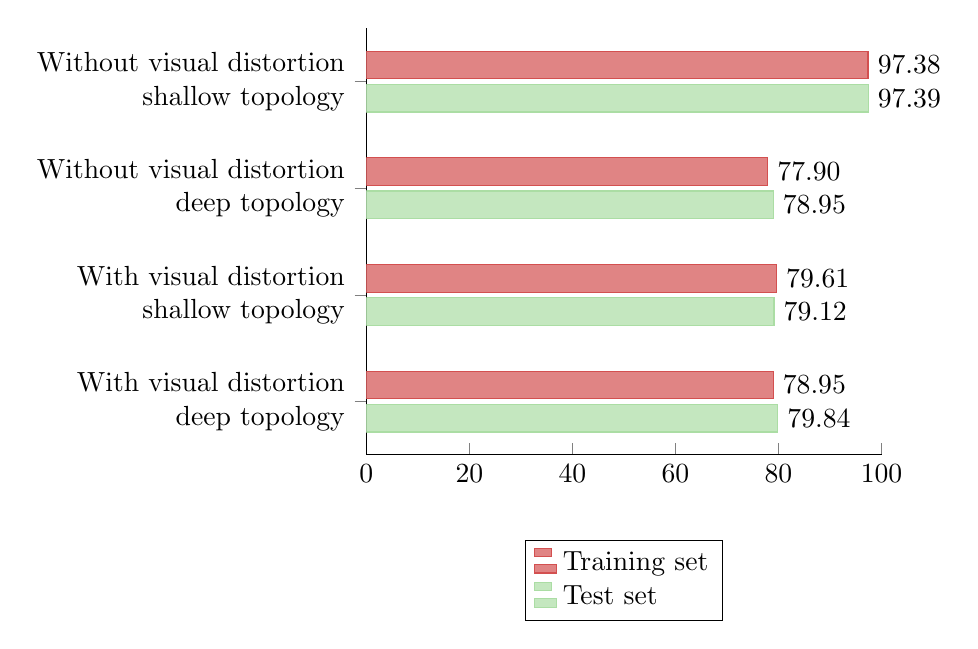
\begin{tikzpicture}
\begin{axis}[
	width=0.67\textwidth,
	height=7cm,
	enlarge y limits={abs=0.5},
	xmin=0,
	xmax=100,
	axis y line*=none,
    axis x line*=bottom,
    xbar,
    reverse legend,
    legend style={at={(0.5,-0.2)},anchor=north},
    yticklabels={
		{Without visual distortion\\shallow topology},
		{Without visual distortion\\deep topology},
		{With visual distortion\\shallow topology},
		{With visual distortion\\deep topology},
	},
	yticklabel style={align=right},
    ytick=data,
    nodes near coords,
    every node near coord/.append style={
		/pgf/number format/fixed zerofill,
		/pgf/number format/precision=2
	},
    ]

% Test set
\addplot [draw=cgreen, fill=cgreen!70] coordinates {
	(97.39,3) % Correct value
	(78.95,2)
	(79.12,1)
	(79.84,0)
};

% Training set
\addplot [draw=cred, fill=cred!70] coordinates {
	(97.38,3) % Correct value
	(77.90,2)
	(79.61,1)
	(78.95,0)
};

\legend{Test set,Training set}
\end{axis}

\end{tikzpicture}
\caption{Accuracy of target detection using angular representation}
\label{fig:angular-acc}
\end{figure}

















































 %DONE
%!TEX root = ../preamble.tex

\hspace{-8mm}
\begin{figure}[H]
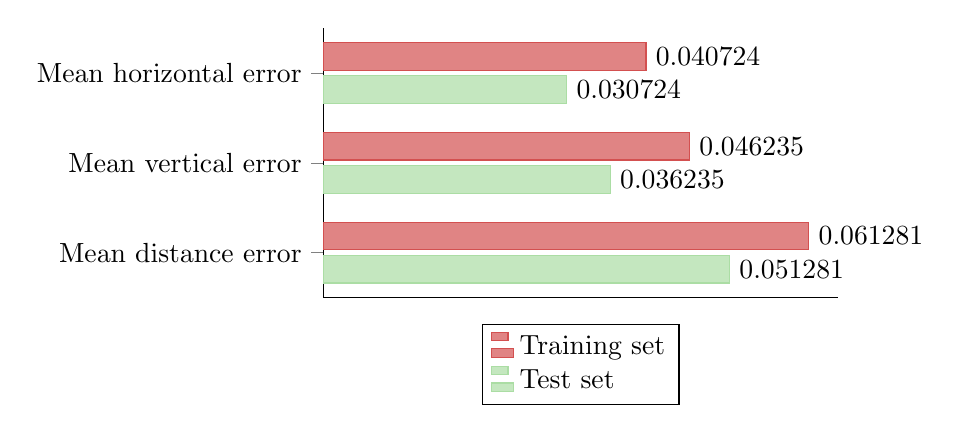
\begin{tikzpicture}
\begin{axis}[
	width=0.67\textwidth,
	height=5cm,
	enlarge y limits={abs=0.5},
	xmin=0,
	xmax=0.065,
	axis y line*=none,
    axis x line*=bottom,
    xbar,
    reverse legend,
    legend style={at={(0.5,-0.1)},anchor=north},
    yticklabels={
		{Mean horizontal error},
		{Mean vertical error},
		{Mean distance error},
	},
	yticklabel style={align=right},
    ytick=data,
	xtick style={draw=none},	
    xticklabels={,,,,,},
    nodes near coords,
    every node near coord/.append style={
		/pgf/number format/fixed zerofill,
		/pgf/number format/precision=6
	},
    ]

% Test set
\addplot [draw=cgreen, fill=cgreen!70] coordinates {
	(0.030724,2) % horizontal error
	(0.036235,1) % vertical error
	(0.051281,0) % distance error
};

% Training set
\addplot [draw=cred, fill=cred!70] coordinates {
	(0.040724,2) % horizontal error
	(0.046235,1) % vertical error
	(0.061281,0) % distance error
};

% DEEP TOPOLOGY. model12.bin. 10,000 samples.
%Mean horizontal error is: 0.040724
%Mean vertical error is: 0.046235
%Mean distance error is: 0.061281
%Accuracy is: 0.979000

\legend{Test set,Training set}
\end{axis}

\end{tikzpicture}
\caption{Angular accuracy of the deep topology without visual distortion}
\label{fig:angular-acc}
\end{figure}
















































 %DONE
%!TEX root = ../preamble.tex

\begin{figure}[h]
\begin{tikzpicture}
\begin{axis}[
	angular-mse,
]

% TEST SET
\addplot [draw=cgreen, fill=cgreen!70] coordinates {
	(0.096121,2) % Correct value
	(0.092301,1) % Correct value
	(0.164209,0) % Correct value
};

% TRAINING SET
\addplot [draw=cred, fill=cred!70] coordinates {
	(0.093103,2) % Correct value
	(0.087807,1) % Correct value
	(0.153207,0) % Correct value
};

\legend{Test set,Training set}
\end{axis}

\end{tikzpicture}
\caption[Mean error of the shallow CNN using AR without visual distortion]{Mean error of the shallow CNN without visual distortion}
\label{fig:angular-mse-nolight-shallow}
\end{figure}
















































 %DONE
%!TEX root = ../preamble.tex

\hspace{-8mm}
\begin{figure}[H]
\begin{tikzpicture}
\begin{axis}[
	angular-mse,
]

\addplot [draw=cgreen, fill=cgreen!70] coordinates {
	(0.161777,2) % Correct value
	(0.172215,1) % Correct value
	(0.163934,0) % Correct value
};
\addplot [draw=cred, fill=cred!70] coordinates {
	(0.162300,2) % Correct value
	(0.171913,1) % Correct value
	(0.161433,0) % Correct value
};

\legend{Test set,Training set}
\end{axis}

\end{tikzpicture}
\caption{Angular accuracy of the deep topology with visual distortion}
\label{fig:angular-acc}
\end{figure}














































 %DONE
%!TEX root = ../preamble.tex



\hspace{-8mm}
\begin{figure}[H]
\begin{tikzpicture}
\begin{axis}[
	angular-mse,
]

\addplot [draw=cgreen, fill=cgreen!70] coordinates {
	(0.179426,2) % Correct value
	(0.186698,1) % Correct value
	(0.169215,0) % Correct value
};
\addplot [draw=cred, fill=cred!70] coordinates {
	(0.179329,2) % Correct value
	(0.186092,1) % Correct value
	(0.165876,0) % Correct value
};

\legend{Test set,Training set}
\end{axis}

\end{tikzpicture}
\caption{Angular accuracy of the shallow topology with visual distortion}
\label{fig:angular-mse-light-shallow}
\end{figure}













































 %DONE

\clearpage
\subsubsection{Feature maps}
\label{sec:featuremaps}
The feature maps shown in figure~\ref{fig:featuremapsvpr}~and~\ref{fig:featuremapsangular} are visualised by scaling the output range of $[0,1]$ of every neuron in the convolutional layers linearly to the grey scale range of $[0,255]$. The leftmost column of feature maps are from the first convolutional layer, and the rightmost is the input to the fully connected layers. As a convolutional layer takes a depth slice of all the previous feature maps as input, their is no apparent connection between the visualised output of the max pooling layer and the following result of the convolutional layer. All of the feature maps are from the same input. Additional feature maps are included in appendix, section~\ref{sec:featuremaps-appendix}. The feature maps from the two different representations are different in both the magnitude and the variance of the output, and the variance. The feature maps from the network estimating the AR has fewer useful feature maps in the last max pooling layer and has a tendency to highlight useless features, such as the weapon overlay, as much as the target.

\begin{figure}[H]
	\begin{scriptsize}
		\sffamily
		\def\svgwidth{\textwidth}
		\input{img/featuremapsvpr.pdf_tex}
	\end{scriptsize}
	\caption[Feature maps for the CNN using VPR]{A small subset of the feature maps produced from running a training example from the lightened arena through the VPR deep convolutional neural network. The feature maps highlight the position of the target.}
	\label{fig:featuremapsvpr}
\end{figure}

\begin{figure}[H]
	\begin{scriptsize}
		\sffamily
		\def\svgwidth{\textwidth}
		\input{img/featuremapsangular.pdf_tex}
	\end{scriptsize}
	\caption[Feature maps for the CNN using AR]{A small subset of the feature maps produced from running a training example from the lightened arena through the AR deep convolutional neural network. The feature maps highlight the position of the target.}
	\label{fig:featuremapsangular}
\end{figure}

\subsubsection{Smaller datasets}
The results shown in figure~\ref{fig:vpr-acc-small-dataset} shows that training with 5015 training examples results in an accuracy of 71.30\%, which is 15.36 percentage points less than the network trained with 130,000 examples. As the accuracy is close to 100\% on the training data, the network clearly overfitted. Whether the networks are trained for the optimal number of  iterations are 

%!TEX root = ../preamble.tex

\begin{figure}[H]
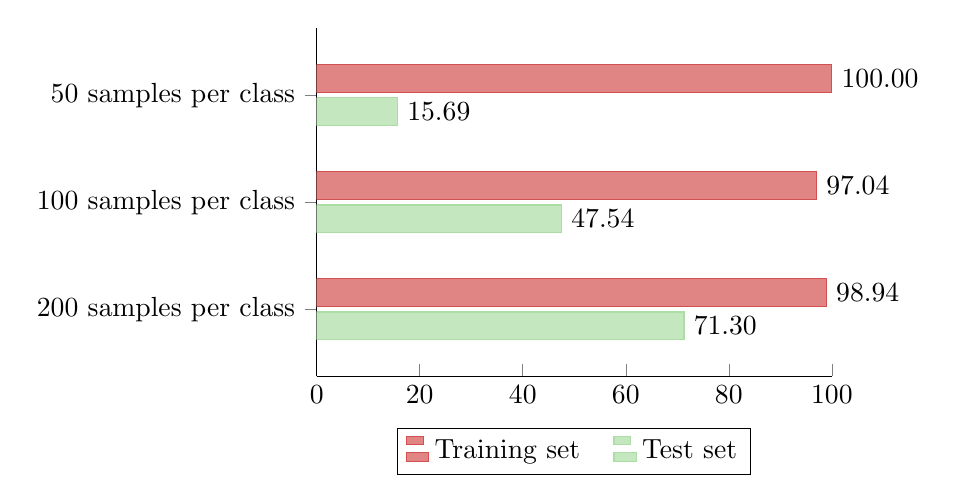
\begin{tikzpicture}
\begin{axis}[%
	width = 0.67\textwidth,
	height = 6cm,
	enlarge y limits={abs=.625},
	xmin=0,
	xmax=100,
	axis y line*=none,
    axis x line*=bottom,
    xbar,
    reverse legend,
    legend style={
		at={(0.5,-0.15)},
		anchor=north,
		/tikz/column 2/.style={
			column sep=10pt,
		},
	},
    yticklabels={
    		{50 samples per class},
		{100 samples per class},
		{200 samples per class},
	},
	yticklabel style={align=right},
	ytick=data,
    nodes near coords,
	every node near coord/.append style={
		/pgf/number format/fixed zerofill,
		/pgf/number format/precision=2
	},
	legend columns=2,
]

\addplot [draw=cgreen, fill=cgreen!70] coordinates {
	(15.690000, 2) 
	(47.540000, 1) 
	(71.300000, 0) 
};
\addlegendentry{Test set}


\addplot [draw=cred, fill=cred!70] coordinates {
	(100.000000, 2) 
	(97.038462, 1) 
	(98.943170, 0) 
};
\addlegendentry{Training set}

\end{axis}

\end{tikzpicture}
\caption{Accuracy of target detection using VPR on small datasets}
\label{fig:vpr-acc-small-dataset}
\end{figure}



%Evaluating model models/deep-small-dataset-50-l2-reg/model120.bin 
%Using db table: trainingDataLightEqualDistribution50PerClass
%Hit rate: 100.000000%

%Evaluating model models/deep-small-dataset-50-l2-reg/model120.bin 
%Using db table: trainingDataLightTestSet 
%Hit rate: 15.690000%



%Evaluating model models/deep-small-dataset-100-l2-reg/model50.bin 
%Using db table: trainingDataLightEqualDistribution100PerClass 
%Hit rate: 97.038462%

%Evaluating model models/deep-small-dataset-100-l2-reg/model50.bin 
%Using db table: trainingDataLightTestSet 
%Hit rate: 47.540000%



%Evaluating model models/deep-small-dataset-200-l2-reg/model50.bin
%Using db table: trainingDataLightEqualDistribution200PerClass
%Hit rate: 98.943170%

%Evaluating model models/deep-small-dataset-200-l2-reg/model50.bin 
%Using db table: trainingDataLightTestSet
%Hit rate: 71.300000%















































\subsection{Neuroevolution experiments}
\label{sec:neuroevolution-experiments-results}
The graphs in figure~\ref{fig:neat-averaged-overall-fitness} and \ref{fig:neat-best-overall-fitness} as well as the graphs included in section~\ref{sec:neuroevolution-graphs} of the appendix are based on evolution with the ground truths as feature representation. The experiments ran for approximately 4 hours each 100 generations. We observe an overall tendency for experiments with the AR to perform better than the experiments with the VPR, both learning faster and reaching a higher fitness. The AR without recoil misses significantly fewer shots than any other approach, as seen in figure~\ref{fig:neat-averaged-missed-shots}. The VPR has fewer unnecessary reloads than the AR, which is the only parameter where it is superior. Non of the approaches  handles recoil well, as visualised in the graphs in figure~\ref{fig:neat-averaged-vpr-recoil-fitness} and \ref{fig:neat-averaged-angular-recoil-fitness}. The AR with recoil eliminates approximately a single target every evaluation, and the VPR manages to hit the target 1 or 2 times. All approaches except VPR without recoil seems to reload with full magazine approximately every second evaluation, as seen in figure~\ref{fig:neat-averaged-wrong-reloads.tex}, which indicates that they do not learn proper reloading behaviour. The decreasing aiming fitness can be attributed to target elimination, as the next target is spawning in a random location.

From inspecting the evolved topologies, we observe different approaches to handling reloading and recoil. The ANNs based on the AR with recoil has a tendency to evolve tap-fire in two different ways. The first one is having a negative weighted recurrent connection from and to the shoot output neuron that allows it to alternate between firing and holding fire. The other one is by slowly aiming away from the target while shooting and stopping when the aiming is too far off. The AR tends to reload when the aim is far off, as this tends to happen when a target is eliminated and a new target appears. The VPR handles recoil by moving to a partition adjacent to the center partition while shooting, and then moving back again to the center partition, creating a short delay in between shots. It tends to associate some of the medium-sized partitions with reloading.

% NEAT GRAPHS
%!TEX root = ../../preamble.tex

\pgfplotstableread{data/neat/ang-mean.dat}{\neatAngularMean}
\pgfplotstableread{data/neat/ang-recoil-mean.dat}{\neatAngularRecoilMean}
\pgfplotstableread{data/neat/vpr-mean.dat}{\neatVPRMean}
\pgfplotstableread{data/neat/vpr-recoil-mean.dat}{\neatVPRRecoilMean}

\begin{figure}[h]
\begin{tikzpicture}[scale=1]
	\begin{axis}[
			height=7.5cm,
			width=0.95\textwidth,
			title=Averaged total fitness over generations,
			xlabel=Generations,
			ylabel=Total fitness,
			ymin = 0,
			ymax = 550,
			xmin = -10,
			xmax = 273,
			restrict x to domain=0:263,
			xticklabel style={rotate=30},
			minor tick num=1,
			legend pos=north west,
			transpose legend,
			legend columns=2,
			legend style={
				/tikz/column 2/.style={
					column sep=10pt,
				}
            },
		]
		\addplot+ [cred, mark=none] table [x={Generation}, y={Fitness}] {\neatAngularMean};
		\addlegendentry{AR - recoil}
		\addplot+ [corange, mark=none] table [x={Generation}, y={Fitness}] {\neatAngularRecoilMean};
		\addlegendentry{AR + recoil}
		\addplot+ [cblue, mark=none] table [x={Generation}, y={Fitness}] {\neatVPRMean};
		\addlegendentry{VPR - recoil}
		\addplot+ [cgreen, mark=none] table [x={Generation}, y={Fitness}] {\neatVPRRecoilMean};
		\addlegendentry{VPR + recoil}
	\end{axis}
\end{tikzpicture}
\caption[Averaged NEAT total fitness]{The total shooting and aiming fitness averaged. Each graph is an average of 3 runs.}
\label{fig:neat-averaged-overall-fitness}
\end{figure} %DONE

%!TEX root = ../../preamble.tex

\pgfplotstableread{data/neat/ang-no-1.txt}{\neatBestAngular}
\pgfplotstableread{data/neat/ang-recoil-2.txt}{\neatBestAngularRecoil}
\pgfplotstableread{data/neat/vpr-no-2.txt}{\neatBestVPR}
\pgfplotstableread{data/neat/vpr-recoil-3.txt}{\neatBestVPRRecoil}

\begin{figure}[H]
\begin{tikzpicture}[scale=1]
	\begin{axis}[
			title=Best overall fitness over generations,
			xlabel=Generations,
			ylabel=Overall fitness,
			ymin = 0,
			ymax = 700,
			xmin = -14,
			xmax = 364,
			restrict x to domain=0:350,
			xticklabel style={rotate=30},
			minor x tick num=1,
			legend pos=north west,
			transpose legend,
			legend columns=2,
			legend style={
				/tikz/column 2/.style={
					column sep=10pt,
				}
            },
		]
		\addplot+ [cred, mark=none] table [x={Generation}, y={Fitness}] {\neatBestAngular};
		\addlegendentry{AR - recoil}
		\addplot+ [corange, mark=none] table [x={Generation}, y={Fitness}] {\neatBestAngularRecoil};
		\addlegendentry{AR + recoil}
		\addplot+ [cblue, mark=none] table [x={Generation}, y={Fitness}] {\neatBestVPR};
		\addlegendentry{VPR - recoil}
		\addplot+ [cgreen, mark=none] table [x={Generation}, y={Fitness}] {\neatBestVPRRecoil};
		\addlegendentry{VPR + recoil}
	\end{axis}
\end{tikzpicture}
\caption[Best NEAT overall fitness]{The best shooting and aiming fitness in a single run from each approach.}
\label{fig:neat-best-overall-fitness}
\end{figure} %DONE

\subsection{The pipeline}
\label{sec:pipeline-results}

The pipeline is the combination of the VRC and the AIC, and it is measured by evaluating fitness over 100 trials with the best performing VRC and the best performing AIC running at 5 TPS. The graph in figure~\ref{fig:neat-cnn-comparison} shows that both the pipeline based on the AR and the VPR are significantly penalised by using the VRC as feature representation provider, decreasing performance by 37.7\% and 73.2\% respectively. Reducing the look sensitivity by 50\% increases the performance of the pipeline, but reduces the performance of the ground truth based AIC.

%!TEX root = ../../preamble.tex

\hspace{-8mm}
\begin{figure}[H]
\begin{center}
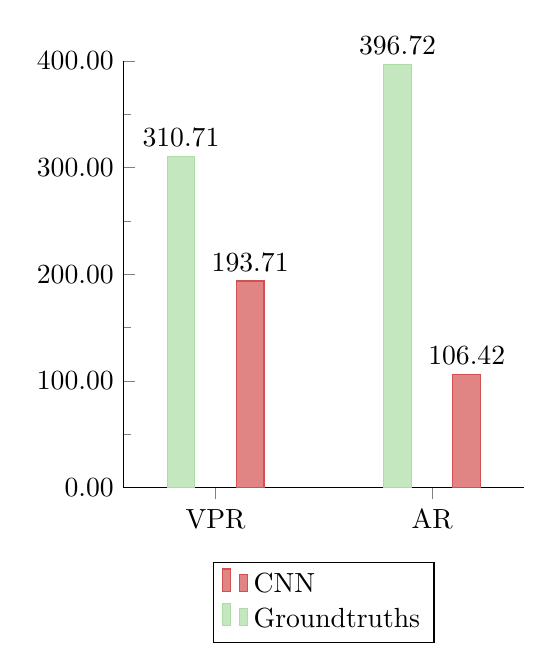
\begin{tikzpicture}
\begin{axis}[
	width=0.55\textwidth,
	height=7cm,
	enlarge x limits={abs=.425},
	ymin=0,
	ymax=400,
	axis y line*=none,
    axis x line*=none,
    ybar = 15pt,
    reverse legend,
	legend style={at={(0.5,-0.175)},anchor=north},
    xticklabels={
    		{AR},
		{VPR},
	},
	xtick=data,
	minor y tick num = 1,
    nodes near coords,
	every node near coord/.append style={
		/pgf/number format/fixed zerofill,
		/pgf/number format/precision=2
	},
]


\addplot [draw=cgreen, fill=cgreen!70] coordinates {
	(1, 396.715369) % Correct value
	(0, 310.706714) % Correct value
};
\addplot [draw=cred, fill=cred!70] coordinates {
	(1, 106.424958) % Correct value
	(0, 193.712533) % Correct value
};

\legend{Groundtruths,CNN}
\end{axis}

\end{tikzpicture}

\caption[Pipeline performance]{Fitness comparison of using the VRC and the groundtruths as features}
\label{fig:neat-cnn-comparison}
\end{center}
\end{figure}


























































































    %!TEX root = ../preamble.tex

\section{Discussion}
\label{sec:discussion}
The discussion is divided into three parts, respectively discussing the VRC, the AIC and the combination.

\subsection{The visual recognition component}
From the results in figure~\ref{fig:vpr-acc}, the CNNs estimating the VPR performed very well. The training examples that the networks failed to predict correctly were either when the target were in between partitions, or behind the weapon overlay, as seen in section \ref{sec:incorrectpredictions} of the appendix. The networks were able to correctly classify images, where we found it difficult to locate the target, as seen in figure~\ref{fig:hardprediction} and in section~\ref{sec:vdexamples} of the appendix and the varying lighting did not seem to cause incorrect predictions.

\begin{figure}[h]
	\begin{scriptsize}
		\sffamily
		\def\svgwidth{\textwidth}
		\input{img/hardprediction.pdf_tex}
	\end{scriptsize}
	\caption[Difficult VPR classification example]{The deep CNN estimating the VPR correctly predicts the class(green square) with a confidence of 55.7\%, with only four pixels of the target being visible. This example was not used for training. The feature maps produced from this example are included in section~\ref{sec:featuremaps-appendix} of the appendix.}
	\label{fig:hardprediction}
\end{figure}

The incorrect predictions of images were the target is present are generally cases were the target could be classified as being in either partition, depending on the exact location of the center of mass of the target. Consequently, such an incorrect prediction does not have a significant impact on an AIC using the incorrect classification to shoot and aim, as some of the target is present in the incorrect partition. These incorrections should therefore be viewed as a natural consequence of the vague classification definition, and not a failure of the optimisation of the model.

Optimising the model with gradient descent proved to be relatively trivial, performing adequately with two distinct network topologies, no regularisation and a very unbalanced distribution of classes. From these observations we conclude that the problem of estimating the VPR is well suited for deep learning. The network with 12 layers and the network with 6 layers performed equally well, but the deeper network did take approximately twice as long to train. However, we can not conclude that increasing the depth does not potentially increase performance if the VPR is applied to harder problems, and the observation should therefore not discourage the use of deeper networks to solve this type of problem. The distribution of classes of training examples is noticeably unbalanced, with more than a 100 times as many classes in the least represented class, as in the most represented class, as seen in table~\ref{tab:enemy-dist}. However, the unbalance does not seem to prevent the network from learning to recognize even the least represented classes. While it seems unlikely that the network can learn to recognize a class from less than 200 training examples, it is possible because the features recognized by the convolutional layer are similar for all the classes, as visualised in figure~\ref{fig:featuremapsvpr}. Hence, the training of less represented classes uses the convolutional filters learned from the more represented classes to optimise the fully connected layers.

The experimentation with training with a smaller volume of data showed that the 5015 examples were insufficient to estimate the VPR to a sufficient accuracy. This suggests that a real world application of the VPR would require a larger amount of labelled data, as we assume that targets in the real world are more visually varied and harder to detect than targets in this game.

The results in the performance paragraph of section~\ref{sec:results-angular-representation} shows varying success with estimating the AR. We observe that the topology of the network has an impact on the error of the horizontal angle, vertical angle and distance, especially when trained without visual distortion. The accuracy of target detection is not affected by the topology, which is not surprising, as it is a strictly easier problem than estimating the VPR. That the topology has a significant influence on the results, leads us to believe, that the problem can be solved with a smaller error if the network topology is improved. Increasing the amount of training data might also yield smaller errors.

The error of the deep network estimating the AR with visual distortion is more than twice as large as the counterpart without visual distortion. Recall that visual distortion both includes dynamic lighting, detailed textures and weapon overlay. This raises the question of how much each of these factors contribute to the error of the network. The visualised errors of figure~\ref{fig:aecollection}, shows that the network has a large error on some examples, where the weapon overlay does not even partially cover the target. Consequently, the two other factors complicates the target detection when estimating the AR. However, it is expected that the weapon overlay adds error in both angles and distance, even if the network functioned optimally. A target in the lower right corner covered by the weapon overlay would be impossible to detect for the VRC, and would in the worst case scenario have an absolute error of 1 in both angles with a theoretically optimal VRC.

The results of the network estimating the VPR with visual distortion indicates, that the network estimating the AR theoretically should be able to approximate the position of the target regardless of visual distortion. The problems of estimating the VPR and the AR have some commonalities, as a VPR can be classified differently if the target is shifted a few pixels. Precision in target detection is therefore necessary in both problems, and the error observed in the network estimating the AR with visual distortion indicates that the network does not have the ability to detect the target with such a precision. However, the deep network estimating the AR without visual distortion proves that estimation of angles with a relatively small error is possible with deep learning. Therefore it is assumed, that the inability of the network  to estimate the AR with an adequate precision is due to insufficient tuning of the learning process, such as the volume or distribution of the training data, the topology of the network or hyper parameters of gradient descent. The network trained by Chenyi Chen et al.\cite{chen} is estimating features similar to the AR, and uses far more training data and trains for more iterations, which also indicates that the network presented by this project is far from optimal. The difference in quality of feature maps, visualised in section~\ref{sec:featuremaps} also indicates, that the convolutional layers of the network estimating the AR is not as functional as the convolutional layers of the network estimating the VPR, which solidifies this assumption. From a theoretical point of view, the difference in the quality of feature maps is not surprising, as the negative log-likelihood cost function optimises better than the euclidean loss cost function used for regression, as described and visualised by Xavier Glorot et al.\cite{DBLP:journals/jmlr/GlorotB10}. Training the network estimating the AR with the convolutional layers of a trained network estimating the VPR could possibly decrease the AR error.

\subsection{The action inferring component}
The results of training the AIC with neuroevolution presented in section~\ref{sec:neuroevolution-experiments-results} show that NEAT is capable of producing networks that can aim and shoot in a FPS game, using both the AR and the VPR. However, the applicability of these networks to other FPS games is heavily challenged by their tendency to learn from the particularities of the FPS game of the project. The distance to the target does not vary much, which the evolved networks exploit to implement reloading and shooting behaviour based on a fixed distance to the target, as the relationship between degrees rotated and the number of pixels that the target shifts on the screen is almost proportional. The network based on AR exploits the fact, that a new target spawns immediately after an elimination by reloading when the target is near the edge of the screen. This tends to result in a single reload as the time it takes to reload is greater than the time it takes to aim directly at the target. The AIC based on the VPR associates specific partitions with reloading. Consequently, none of the AICs learns generalisable reloading behaviour. Proper reloading behaviour requires either information about the number of shots left or long-term memory, none of which the AIC possess. The observations are therefore not surprising from a theoretical point of view.

The inability of the networks to develop human-like tap-fire is possibly because of the limited training time. While we can conclude that 250 generations are not enough to develop this behaviour, we can not conclude that this approach is unable to develop tap-fire behaviour given enough time.

Neuroevolution evolves networks that are tailored to the task that they are evaluated on, and as our FPS game lacks variation, the networks does not learn much general applicable logic, except aiming and shooting without recoil. The best way to investigate the potential of NEAT in the domain of FPS games are to develop more varied evaluations that resembles modern FPS games. This is a significant shortcoming of the project, and optimisation of this area is recommended if the combination approach should be taken further.


\subsection{The pipeline}
The results in figure~\ref{fig:neat-cnn-comparison} show a significant difference between the reduction in performance from using a VRC with the AR and the VPR. The pipeline using a VRC estimating the AR clearly performs worse, and this observation corresponds with the performance evaluation of the individual VRCs in section~\ref{sec:results-angular-representation}. The estimation of the AR is far too inaccurate for the AIC to successfully infer an adequate action, and has its fitness reduced by 73.2\% when using the VRC. The weapon overlay covering the target reduces performance for both approaches, but this factor does not explain the entire 37.7\% fitness reduction from using a VRC with the VPR. From detailed examination of running the pipeline with a VRC estimating the VPR, we observed that the combination of low TPS and classification uncertainty when the target is in between partitions was a challenge. As the AIC is trained with the ground truths, assuming that the target is within a partition after a number of time steps given a specific AIC output is relatively safe. However, when the estimation of the VPR is inaccurate when the target is in between partitions, this assumption does not hold and can lead to unwanted behaviour. The consequence of this behaviour is amplified by the fact, that the AIC using the VPR associates specific partitions with reloading, penalising inaccurate partitioning classification. That the reduction in fitness can be attributed to this problem is substantiated by the increase in pipeline performance from reducing the look sensitivity, as seen in figure~\ref{fig:neat-cnn-comparison}.

The observations from the pipeline experiments harmonises well with the observations from the VRC experiments, and indicates that the VPR is easier estimated by deep learning than the AR.

Running the agent with the pipeline proved performance intensive, and the overall performance of the agent is definitely reduced by running with only 5 TPS. While the experiments failed to explore how well the combination could perform, they prove that it is possible for the combination to learn to aim and shoot with the VPR. We definitely believe that the approach can work for the AR, but the AR pipeline performance is not convincing enough to support any conclusions to this approach.

\subsection{Applications in real world robotics}


Generalising the feature representation to represent multiple targets...

Security cameras, interception missile system

    \section{Future work}
The integration of the CNN and the ANN evolved with neuroevolution involved binarising the output of the CNN, such that the CNN mimics the output that the evolved ANN was trained with. However, this does not explore the potential of the evolved ANN to use the analog output of the CNN, which might make the integration work better. The probability distribution of the features vector of the visual partitioning representation reveals additional information about the position of the target, as an uncertainty usually means that the target is between two partitions. Consequently, we believe that evolving the ANN with the analog output of the CNN could result in even better performance than using the ground truths directly.

Compare our approach with vizdoom in the domain of doom.
    \section{Conclusion}
It was nice working with u guys!
	
	\newpage
	
	\begin{appendices}
		%!TEX root = ../preamble.tex

\section{Technical Description}
Bla bla bla

\subsection{Hardware used for training}
\label{sub:hardware}
All training of the CNN was done on a server, at the IT University of Copenhagen, with the following specs:

\begin{description}
	\item [CPU] Intel\textsuperscript{\textregistered} Core\textsuperscript{\texttrademark} i7-5820K
	\item [GPU] 2x GeForce\textsuperscript{\textregistered} GTX TITAN X
	\item [RAM] 32 GB HyperX Fury DDR4 2400 C15
\end{description}	

\noindent
Each training experiment was done using one of the GPUs and up to 12 GB of RAM allowing for two simultaneous runs.

\subsection{Bridging between Unity and DL4J}\todo{Move this to Theory?}
The game used is made using the game engine Unity, where it is possible to interface with the game using either C\#, JavaScript, Boo or Unity Script.

The convolutional neural network is trained using DL4J \todo{Has DL4J been introduced at this point?}, which is written in Java.
It is unfortunately not possible to interface with the game using Java. Somehow the game has to communicate with a convolutional neural network.

\section{Figures}

\begin{figure}[H]
	\begin{scriptsize}
		\sffamily
		\def\svgwidth{\textwidth}
		\input{img/grid.pdf_tex}
	\end{scriptsize}
	\caption{Ids of the 3, 3, 3 partitioning scheme}
	\label{fig:ids}
\end{figure}

\section{Incorrect predictions}
\label{sec:incorrectpredictions}
The following examples are incorrect predictions by the deep visual partitioning convolutional neural network. The green squares mark the ground truths, and the red squares mark the wrong predictions. Absence of either the red or the green square means that either the the prediction  or the ground truth is that no target is present on the screen.

\begin{figure}[H]
	\begin{center}
	\begin{scriptsize}
		\sffamily
		\def\svgwidth{0.95\textwidth}
		\input{img/failcollection1.pdf_tex}
	\end{scriptsize}
	\label{fig:failcollection1}
	\end{center}
\end{figure}


\begin{figure}[H]
	\begin{center}
	\begin{scriptsize}
		\sffamily
		\def\svgwidth{0.95\textwidth}
		\input{img/failcollection2.pdf_tex}
	\end{scriptsize}
	\label{fig:failcollection2}
	\end{center}
\end{figure}

\section{Angular representation error}
\label{sec:angular-error}
\begin{figure}[H]
	\begin{center}
	\begin{scriptsize}
		\sffamily
		\def\svgwidth{1\textwidth}
		\input{img/angularError.pdf_tex}
	\end{scriptsize}
	\label{fig:angularerror}
	\caption[AR mean error visualised]{The blue box marks the average error margins for horizontal and vertical angles for the deep CNN without visual distortion, while the red box marks the same error for the shallow CNN.}
	\end{center}
\end{figure}

\section{Visually distorted examples}
\label{sec:vdexamples}
\begin{figure}[H]
	\begin{center}
	\begin{scriptsize}
		\sffamily
		\input{img/vd1.pdf_tex}
	\end{scriptsize}
	\label{fig:vd1}
	\caption[Visually distorted example]{The deep CNN estimating the VPR correctly predicts the class(id 0) with a confidence of 71.9\%.}
	\end{center}
\end{figure}

\begin{figure}[H]
	\begin{center}
	\begin{scriptsize}
		\sffamily
		\input{img/vd2.pdf_tex}
	\end{scriptsize}
	\label{fig:vd2}
	\caption[Visually distorted example]{The deep CNN estimating the VPR correctly predicts the class(id 4) with a confidence of 78.0\%.}
	\end{center}
\end{figure}

\begin{figure}[H]
	\begin{center}
	\begin{scriptsize}
		\sffamily
		\input{img/vd3.pdf_tex}
	\end{scriptsize}
	\label{fig:vd3}
	\caption[Visually distorted example]{The deep CNN estimating the VPR incorrectly predicts the class(id 2) with a confidence of 58.9\%. The correct class has id 4.}
	\end{center}
\end{figure}
	\end{appendices}
	
	\clearpage
	\bibliographystyle{ieeetr}
	\bibliography{bibliography}
\end{document}















































